\chapter{Experimenty} \label{cha:experiments}

Táto kapitola je venovaná popisu a vyhodnoteniu experimentov navrhnutých za cieľom vyhodnotenia úspešnosti systému popísaného v~predchádzajúcej kapitole. Na začiatok porovnáme výsledky nášho systému s~referenčným článkom, aby sme overili jeho funkčnosť. Následne vyhodnotíme rôzne prístupy hodnotenia výslovnosti vrátane ich modifikácii a vyberieme metódy s~najlepšími výsledkami. Na záver nad vybranými metódami overíme, aký bude mať vplyv použitie akustického modelu trénovaného na viacerých jazykoch na výslednú úspešnosť pri hodnotení výslovnosti.

\section{Spôsob vyhodnotenia experimentov} \label{sec:vyhodnotenie-experimentov}

Pri vyhodnotení experimentov budeme uvažovať len chyby výslovnosti spočívajúce vo vypúšťaní a zámene foném. Na detekciu chýb spôsobených vložením jednej alebo viacerých foném sa totiž používajú odlišné prístupy, napr. rozšírené rozpoznávacie siete (\textit{Extended Recognition Networks}) \cite{Arora2018}. K~určeniu druhu chyby je potrebné porovnať kanonické a skutočné prepisy. 

Úspešnosť uvažovaných metód vyhodnotíme pomocou tzv. miery chybného prijatia (\textit{False Acceptance Rate}, FAR) a miery chybného odmietnutia (\textit{False Rejection Rate}, FRR), kde FAR udáva pomer medzi počtom zle vyslovených foném klasifikovaných ako správne vyslovené k~celkovému počtu zle vyslovených foném a FRR je naopak pomer medzi počtom správne vyslovených foném klasifikovaných ako nesprávne vyslovené k~celkovému počtu správne vyslovených foném. Keďže sa tieto hodnoty líšia v~závislosti na použitom prahu, vykreslíme si ich vzájomnú závislosť. Takto získame graf, ktorý sa zvykne označovať ako ROC krivka. Pre číselné porovnanie metód použijeme tzv. rovnakú mieru chyby (\textit{Equal Error Rate}, ERR), ktorá je rovná hodnote FAR, resp. FRR, keď je FAR a FRR totožné, t.j. $\text{EER} := \text{FAR} = \text{FRR}$.

Výsledky v~prípade použitia neurónovej siete bývajú do určitej miery závislé na jej počiatočnej inicializácii pri trénovaní. Nakoľko v~našom prípade inicializujeme sieť náhodne, je vhodnejšie uvádzať strednú hodnotu spolu s~rozptylom určenú z~niekoľkých klasifikátorov s~rôznou inicializáciou. Toto nám umožní objektívnejšie porovnať rôzne metódy využívajúce neurónové siete. Vo všetkých prípadoch bude táto hodnota určená z~10 klasifikátorov s~náhodnou inicializáciou. Obdobný postup použijeme pri grafoch závislosti FAR a FRR, kde určíme tieto hodnoty zo zpriemerovaných rozhodnutí od všetkých 10 klasifikátorov.

\section{Parametre experimentov}

Navrhnutý systém realizujeme v~toolkite Kaldi \cite{Kaldi}, čo je open-source nástroj vyvinutý k~rozpoznávaniu reči. Napriek tomu, že obsahuje aj natívnu implementáciu neurónových sietí potrebných k~akustickému modelovaniu, rozhodli sa pre ich implementáciu v~nástroji Keras \cite{keras}. Ten totiž podporuje jednoduchšie a flexibilnejšie modifikácie realizovanej neurónovej siete, čo využijeme v~niektorých experimentoch.

\subsection*{Dataset}

K~experimentom využijeme nenatívny dataset ISLE, ktorý rozdelíme na trénovaciu a testovaciu sadu, kde pre každý L1 jazyk v~datasete použijeme nahrávky od 19 rečníkov na trénovanie a 4 rečníkov na testovanie. Ďalej ale už nahrávky podľa jazykov rozlišovať nebudeme, pretože samostatne by na trénovanie nebolo dostatok dát. Rozdelenie datasetu je v~súlade s~referenčnou prácou \cite{Arora2017}, čo nám umožní jednoduché porovnanie dosiahnutých výsledkov. Po rozdelení majú nahrávky v~trénovacej sade dĺžku 8 hodín a 24 minút a v~testovacej sade 1 hodinu a 34 minút. Zoznam rečníkov v~jednotlivých sadách sa nachádza v~tabuľke \ref{tab:train-test-sets}. Pri trénovaní neurónovej siete použijeme aj validačnú sadu, ktorá pozostáva z~troch rečníkov trénovacej sady -- SESS0131, SESS0138 a SESS0186.

Nakoľko nebudeme pri experimentoch uvažovať chyby založené na vkladaní foném, rozšírime kanonický prepis o~vložené fonémy nachádzajúce sa v~skutočnom prepise. Ak by sme tento krok vynechali, nútené zarovnania na kanonický prepis by mohli viesť na segmenty pozostávajúce z~rámcov odpovedajúcich viacerým fonémam.

\begin{table}[ht]
\centering
\begin{tabular}{@{}l|lllll@{}}
\toprule
Testovacia sada & \multicolumn{5}{l}{Trénovacia sada}                  \\ \midrule
SESS0006        & SESS0012 & SESS0183 & SESS0191 & SESS0126 & SESS0134 \\
SESS0011        & SESS0021 & SESS0184 & SESS0192 & SESS0127 & SESS0135 \\
SESS0015        & SESS0161 & SESS0185 & SESS0193 & SESS0128 & SESS0136 \\
SESS0020        & SESS0162 & SESS0186 & SESS0003 & SESS0129 & SESS0137 \\
SESS0041        & SESS0163 & SESS0187 & SESS0040 & SESS0130 & SESS0138 \\
SESS0121        & SESS0164 & SESS0188 & SESS0123 & SESS0131 & SESS0140 \\
SESS0122        & SESS0181 & SESS0189 & SESS0124 & SESS0132 &          \\
SESS0139        & SESS0182 & SESS0190 & SESS0125 & SESS0133 &          \\ \bottomrule
\end{tabular} 
\caption{Rozdelenie ISLE datasetu na testovaciu a trénovaciu sadu, pričom údaje v~tabuľke predstavujú identifikátory jednotlivých rečníkov.} \label{tab:train-test-sets}
\end{table}


\subsection*{Akustický model} 

Vstupom DNN akustického modelu je 23 fbank príznakov s~kontextom $\pm 5$ rámcov. Príznaky sú pred tým normalizované, aby mali nulovú strednú hodnotu a jednotkový rozptyl. 
DNN pozostáva z~3 skrytých vrstiev, ktoré sú tvorené 512 neurónmi s~ReLU aktivačnou funckiou. Výstupné neuróny so soft-max prenosovou funkciou určujú pravdepodobnosť stavov monofónneho, resp. trifónneho modelu. Jednotlivé modely zodpovedajú 41 kanonickým fonémam, tichu a nakoniec špeciálne zavedenej fonéme, do ktorej je združených 8 foném pochádzajúcich z~natívneho jazyka rečníkov. % Trifónový model pozostáva zo zlúčených trifónov získaných zhľukovaním pomocou rozhodovacieho stromu. 

Trénovanie prebieha na fonémových zarovnaniach vzhľadom na skutočný prepis. K~zarovnaniu je použitý GMM-HMM model natrénovaný na tých istých dátach. Na vstup GMM-HMM modelu je privedených 39 MFCC+$\Delta$+$\Delta\Delta$ príznakov. DNN je trénovaná s~využitím Adam optimalizátoru nad trénovacími dávkami (mini-batches) o~veľkosti 256 rámcov. Ako objektívna funkcia je zvolená kategorická krížová entropia. K~zabráneniu pretrénovania je použitý 10\,\% dropout. Miera rýchlosti trénovania (\textit{learning rate}) je $0{,}001$ do doby, než sa hodnota objektívnej funkcie na validačnej dátovej sade prestane zlepšovať, maximálne však po dobu 15 epoch. Potom sa s~každou epochou zmenšuje o~polovicu a trénovanie končí, ak sa hodnota objektívnej funkcie nezlepšila počas 10 epoch. 

\subsection*{Určovanie fonologických rysov}

Extrakciu fonologických rysov zabezpečuje DNN s~totožnou topológiou a parametrami ako v~prípade akustického modelu. Jediný rozdiel je vo výstupnej vrstve, ktorá má softmax aktivačnú funkciu, a tvorí ju $19$ neurónov, ktoré odpovedajú fonologickým rysom a tichu. 
Počas trénovania sa využívajú zarovnania na kanonický prepis získané pomocou monofónového GMM-HMM modelu, ktoré sa prevádzajú na fonologické rysy pomocou tabuľky \ref{tab:phonolog-features-set}.

\subsection*{Priama klasifikácia výslovnosti}

Na priamu klasifikáciu výslovnosti použijeme jednak jednoduchú neurónovú sieť s~dopredným šírením a taktiež rekurentnú neurónovú sieť s~LSTM architektúrou. Jednoduchá neurónová sieť sa skladá z~jedinej skrytej vrstvy, ktorú tvorí $512$ neurónov s~ReLU aktivačnou funkciou. LSTM neurónovú sieť tvorí 512 jednotiek, pričom ich architektúra je v~súlade s~popisom uvedeným v~kapitole \ref{cha:neural-networks}. 

V~závislosti na experimentoch sú na vstup neurónových sieti privádzané logaritmické hodnoty vierohodností HMM stavov, alebo pravdepodobnosti fonologických rysov, normalizované na nulovú strednú hodnotu a jednotkový rozptyl. V~prípade LSTM neurónovej siete tvoria príznakový vektor príznaky určené zo všetkých rámcov uvažovaného segmentu, pričom u~jednoduchej neurónovej siete je vstupom len priemerná hodnota týchto príznakov. Pre obe neurónové siete platí, že aktivačná funkcia výstupnej vrstvy je logistická sigmoida.

Trénovanie prebieha nad segmentmi získanými núteným zarovnaním pomocou GMM-HMM modelu voči kanonickému prepisu. S~trénovania sú vynechané segmenty, ktoré zodpovedajú vloženým fonémam, nakoľko tento druh chýb neuvažujeme. Riadenie trénovania zabezpečuje optimalizačný algoritmus Adam s~veľkosť trénovacej dávky (\textit{mini-batch}) $256$ vzoriek. Objektívnou funkciou je krížová entropia a droput je na úrovni $10\,\%$. Miera rýchlosti trénovania je $0{,}001$ počas prvých troch epoch, potom sa s~každou epochou znižuje o~polovicu. Trénovanie končí, ak sa za posledné 4 epochy nezlepšila hodnota objektívnej funkcie na validačných dátach. 

\section{Porovnanie základných metód s~referenčnou prácou}

Za účeľom overenia funkčnosti nami navrhnutého systému porovnáme dosiahnuté výsledky s~referenčným systémom od Arora a kol. \cite{Arora2017}. Porovnávať budeme trojicu metód postavených na monofónovom akustickom modeli, ktoré boli použité aj v~referenčnej práci. Sú nimi štandardné GOP skóre (STD GOP), dopredná neurónová sieť natrénovaná nad vierohodnosťami HMM stavov (NN HMM) a nakoniec dopredná neurónová sieť rozhodojúca na základe pravdepodobností fonologických rysov (NN PFeats). 

V~prípade metód priamej klasifikácie sme oproti referenčnému systému zaviedli niekoľko zmien. Namiesto strednej kvadratickej chyby v~pri oboch neurónových sieťach využívame kategorickú krížovú entropiu, ktorá je na tento typ problému vhodnejšia. V~dôsledku tohto kroku je možné očakávať mierne lepšie výsledky. Ďalšia zmena spočíva v~inom type použitej neurónovej siete určujúcej fonologické rysy. Sieť použitá v~referenčnom systéme je súčasne trénovaná na dve úlohy -- určovanie fonologických rysov aj HMM stavov. Keďže naša neurónová sieť je trénovaná len na prvej z~nich, dá sa predpokladať, že dosiahneme horší výsledok. Rozdiel by však nemal byť výrazný. Poslednou odlišnosťou je normalizácia príznakov (vierohodností HMM stavov aj pravdepobností fonologických rysov) na nulovú strednú hodnotu a jednotkový rozptyl. Ukázalo sa totiž, že najmä v~prípade nenormovaných vierohodností neurónová sieť horšie konverguje k~riešeniu, alebo dokonca pri použití trifónového modelu nekonverguje vôbec.

Dosiahnuté výsledky je možné v~podobe ROC kriviek vidieť na obrázku \ref{fig:roc-basic-methods} a ich vyjadrenie pomocou miery rovnakej chyby (EER) v~tabuľke \ref{tab:eer-basic-methods}, kde sa zároveň nachádzajú aj výsledky referenčného systému. Hodnoty ukazujú, že nami zostrojený systém je funkčný, aj keď sme pri metóde využívajúcej fonologické rysy dosiahli mierne horší výsledok. To je však v~súlade s~hore uvedeným predpokladom o~vplyve viacúlohového učenia.

Výrazne nižšiu chybu vykázal systém u~GOP skóre a klasifikátora využívajúceho pravdepodobnosti HMM stavov. Pri druhej menovanej metóde bolo zlepšenie až $4{,}23$ percentuálnych bodov. Takýto výrazný rozdiel môže byť spôsobený dvojicou faktorov, a to použitím odlišnej objektívnej funkcie a normalizovaním príznakov. Oboje totiž výrazne prispieva ku konvergencii k~optimálnemu riešeniu, čo nemuselo byť prípadom referenčného systému.

Poslednou metódou, ktorú sme porovnávali, je štandardné GOP skóre. Rozdiel medzi systémami je tentokrát ešte značnejší, so zlepšením na úrovni $5{,}65$ percentuálnych bodov. K~zdôvodneniu takéhoto výsledku nám však v~prípade referenčného systému chýba dostatok informácii. Predpokladáme však, že nimi implementovaný akustický model mohol byť nesprávne optimalizovaný, čo by vysvetlovalo aj výsledok u~NN HMM klasifikátora.

%Aj to však platí len v prípade, keď porovnáme strednú hodnotu určenú z viacerých inštancií klasifikátora. Ak totiž zoberieme v úvahu najlepší dosiahnutý výsledok (EER = $28.20 \%$), tak aj 


\begin{table}[h!]
    \centering
    \begin{tabular}{@{}llll@{}}
    \toprule
    EER {[}\%{]}                       & STD GOP & NN HMM           & NN PFeats        \\ \midrule
    Navrhnutý systém                   & $\bm{33{,}35}$ & $\bm{27{,}57} \pm 0{,}16$ & $28{,}49 \pm 0{,}14$ \\
    Referenčný systém \cite{Arora2017} & $39{,}00$ & $31{,}80$          & $\bm{28{,}30}$          \\ \bottomrule
    \end{tabular}
    \caption{Dosiahnuté výsledky pomocou základných metód -- štandardná GOP metóda (STD GOP), neurónové siete klasifikujúce na základe HMM vierohodností (NN HMM) a na základe pravdepodobností fonologických rysov (NN Pfeats).} \label{tab:eer-basic-methods}
    \end{table}

\begin{figure}[h!]
    \centering
    % This file was created by matplotlib2tikz v0.6.18.
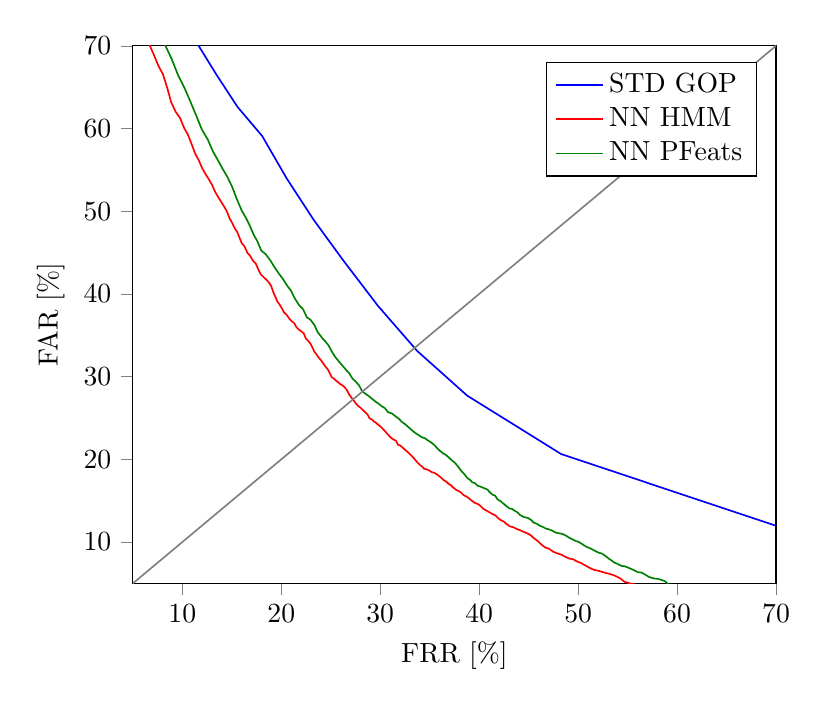
\begin{tikzpicture}

\begin{axis}[
tick align=outside,
tick pos=left,
x grid style={white!69.01960784313725!black},
xlabel={FRR [\%]},
xmin=5, xmax=70,
y grid style={white!69.01960784313725!black},
ylabel={FAR [\%]},
ymin=5, ymax=70,
legend pos=north east,
width=9.75cm,
legend cell align={left},
]

\addplot [semithick, blue]
table {%
100 0
48.295262743333 20.6355591311344
38.7794906417614 27.7152051488335
33.7384194141255 33.1053901850362
29.7588237500469 38.5760257441673
26.2443269194704 44.0868865647627
23.2774464573722 48.9541432019308
20.5393646149807 53.9823008849557
18.0750909568283 59.0909090909091
15.5920633134541 62.5905068382944
13.5028693597389 66.4119066773934
11.5712088818874 70.152855993564
9.80083267694385 73.9742558326629
8.47680132028056 77.1118262268705
7.18652713701662 80.1287208366854
6.03503244439443 82.4215607401448
5.00731405423653 84.3523732904264
4.11462435767601 85.880933226066
3.37196654289036 87.5703942075624
2.76058662465774 89.0185036202735
2.28048460297813 90.2654867256637
1.8566445369641 91.2308930008045
1.52657439705938 91.9147224456959
1.23776302464274 92.8399034593725
1.02021679606916 93.3628318584071
0.8551817261168 94.2075623491553
0.697648250253179 94.8109412711183
0.573871947788905 95.3740949316171
0.468849630546491 96.0176991150443
0.363827313304077 96.2590506838295
0.296312966505382 96.7417538213998
0.262555793106035 97.3451327433628
0.225047822662316 97.6267095736122
0.202543040396084 97.98873692679
0.191290649262968 98.2300884955752
0.180038258129853 98.592115848753
0.161284272907993 98.8736926790024
0.131277896553018 98.994368463395
0.108773114286786 99.0748189863234
0.0975207231536701 99.1552695092518
0.0900191290649263 99.2759452936444
0.0787667379318105 99.4368463395012
0.0750159408874386 99.597747385358
0.0562619556655789 99.597747385358
0.0412587674880912 99.597747385358
0.0337571733993474 99.597747385358
0.0300063763549754 99.7184231697506
0.0300063763549754 99.7586484312148
0.0262555793106035 99.798873692679
0.0262555793106035 99.8390989541432
0.0187539852218596 99.9597747385358
0.0187539852218596 100
0.0150031881774877 100
0.0112523911331158 100
0.00750159408874386 100
0.00375079704437193 100
}; \addlegendentry{STD GOP}

\addplot [semithick, red]
table {%
0 100
2.50928322268482 85.2373290426388
3.66827950939575 81.2148028962188
4.66974232024305 77.1922767497989
5.3711413675406 74.8994368463395
5.92625933010765 72.3250201126307
6.58264881287274 70.3942075623492
7.11151119612918 68.946098149638
7.61411800007502 67.4979887369268
8.04170886313342 66.5728077232502
8.50305689959116 64.8028962188254
8.87063500993961 63.1938857602574
9.32823224935299 62.0273531777957
9.79333108285511 61.2228479485117
10.2171711488691 59.9758648431215
10.5734968680845 59.2518101367659
10.9860845429654 57.9646017699115
11.3011514946926 56.9589702333065
11.6499756198192 56.1946902654867
11.9987997449458 55.2292839903459
12.3363714789393 54.5052292839903
12.6626908217996 53.9018503620273
13.0077641498819 53.1777956556718
13.3190803045647 52.3330651649236
13.6566520385582 51.6492357200322
13.9379618168861 51.1263073209976
14.2680319567908 50.4827031375704
14.54184014103 49.8793242156074
14.7706387607367 49.1552695092518
15.0181913656652 48.6323411102172
15.2957503469487 47.9485116653258
15.5583061400548 47.4658085277554
15.7570983834065 46.8624296057924
16.0009001912906 46.1383748994368
16.2709575784854 45.776347546259
16.5785229361239 44.9718423169751
16.8523311203631 44.6098149637973
17.1261393046022 44.0466613032985
17.4187014740632 43.6846339501207
17.6850080642136 42.9605792437651
17.9175574809647 42.3974255832663
18.1801132740707 42.0756234915527
18.465173849443 41.7538213998391
18.7427328307265 41.3917940466613
18.9715314504332 40.9895414320193
19.181576084918 40.2654867256637
19.3503619519148 39.7827835880933
19.6204193391096 39.0587288817377
19.82671317655 38.7369267900241
20.048010202168 38.2944489139179
20.2730580248303 37.7715205148833
20.5581186002025 37.4497184231698
20.7869172199092 37.0474658085278
21.0644762011928 36.68543845535
21.3307827913432 36.4440868865648
21.5220734406061 36.0016090104586
21.7508720603128 35.7200321802092
22.0171786504632 35.478680611424
22.2684820524361 35.2373290426388
22.478526686921 34.6339501206758
22.7485840741157 34.271922767498
22.9473763174675 33.9903459372486
23.1574209519523 33.5076427996782
23.3412100071265 33.0249396621078
23.5512546416113 32.7031375703942
23.780053261318 32.3008849557522
24.0426090544241 31.9388576025744
24.2526536889089 31.5768302493966
24.4889539027043 31.1745776347546
24.6989985371892 30.8930008045052
24.8865383894078 30.450522928399
25.0815798357151 29.9678197908286
25.3103784554218 29.7666934835076
25.494167510596 29.5655671761866
25.7529725066577 29.3242156074014
26.0192790968081 29.0426387771521
26.2255729342485 28.9219629927595
26.4356175687334 28.6806114239743
26.6306590150407 28.3588093322607
26.8932148081467 27.7956556717619
27.1070102396759 27.4336283185841
27.3170548741608 27.1520514883347
27.4858407411575 26.8302493966211
27.7221409549529 26.5084473049075
27.9771951539702 26.2670957361223
28.2547541352537 25.9452936444087
28.4798019579161 25.7039420756235
28.7198529687559 25.4223652453741
28.9336484002851 24.9396621078037
29.1774502081692 24.8189863234111
29.3649900603878 24.5776347546259
29.5862870860058 24.4167337087691
29.8038333145793 24.1753821399839
29.9951239638423 24.0144810941271
30.193916207194 23.7731295253419
30.415213232812 23.4915526950925
30.6590150406961 23.1697506033789
30.8765612692697 22.8881737731295
31.131615468287 22.5663716814159
31.3979220584374 22.3652453740949
31.6042158958779 22.2445695897023
31.7992573421852 21.7618664521319
32.00930197667 21.6814159292035
32.2568545815986 21.4400643604183
32.5006563894828 21.1584875301689
32.7069502269232 20.9573612228479
32.9695060200293 20.6757843925986
33.2620681894903 20.3137570394208
33.4758636210195 20.0321802091714
33.7271670229924 19.6701528559936
33.9859720190541 19.34835076428
34.2147706387607 19.147224456959
34.4360676643787 18.8656476267096
34.6761186752185 18.7851971037812
34.9499268594576 18.6645213193886
35.1862270732531 18.4633950120676
35.437530475226 18.3829444891392
35.6850830801545 18.2220434432824
35.9138816998612 18.0209171359614
36.1576835077454 17.7795655671762
36.4052361126739 17.4979887369268
36.6865458910018 17.2968624296058
36.8778365402648 17.0555108608206
37.1178875511046 16.8946098149638
37.3579385619444 16.6130329847144
37.6467499343611 16.331456154465
37.9130565245115 16.1705551086082
38.1456059412625 16.0096540627514
38.4456697048123 15.6476267095736
38.6857207156521 15.526950925181
38.9820336821575 15.2855993563958
39.2483402723079 15.0040225261464
39.582161209257 14.722445695897
39.8709725816736 14.6017699115044
40.1410299688684 14.3604183427192
40.4073365590188 14.0386162510056
40.7411574959679 13.7972646822204
41.044972056562 13.5961383748994
41.337534226023 13.3950120675784
41.630096395484 13.2341110217216
41.9376617531225 12.8720836685438
42.2114699373617 12.6307320997586
42.5040321068227 12.4698310539019
42.7515847117512 12.1882542236525
43.0929072427891 11.9066773934031
43.4679869472263 11.7860016090105
43.7943062900866 11.5848753016895
44.1581336033907 11.4239742558327
44.5144593226061 11.2228479485117
44.8520310565995 11.0619469026549
45.1783503994599 10.8608205953339
45.5084205393646 10.4987932421561
45.9435129965118 10.0965406275141
46.3298450920821 9.65406275140788
46.6936724053861 9.33226065969429
47.0987584861783 9.17135961383749
47.4550842053936 8.84955752212389
47.8564194891414 8.6484312148029
48.2877611492442 8.4875301689461
48.6665916507258 8.2461786001609
49.1016841078729 8.0048270313757
49.5030193916207 7.9243765084473
49.8330895315254 7.68302493966211
50.2681819886726 7.48189863234111
50.6845204605979 7.20032180209171
51.1608716852331 6.87851971037812
51.603465736469 6.63716814159292
52.0948201492817 6.51649235720032
52.6274333295825 6.31536604987932
53.1675481039721 6.15446500402253
53.6926596901842 5.95333869670153
54.2290236675294 5.63153660498793
54.6978732980758 5.18905872888174
55.2717452458647 4.98793242156074
55.8906267581861 4.82703137570394
56.4982558793744 4.58567980691874
57.1846517384944 4.34432823813355
57.9273095532801 4.10297666934835
58.6212070064889 3.86162510056315
59.3151044596977 3.70072405470636
60.0615130715277 3.49959774738536
60.7779153070027 3.41914722445696
61.5280747158771 3.29847144006436
62.4095120213045 3.05711987127916
63.3247065001313 2.81576830249397
64.3261693109786 2.69509251810137
65.2788717602491 2.53419147224457
66.3028393533626 2.29283990345937
67.4505832489404 2.17216411906677
68.6245827238288 2.05148833467418
69.9711188627583 1.68946098149638
71.4376805071078 1.48833467417538
73.1030343948089 1.32743362831858
74.8546566145306 0.884955752212389
76.8163234687371 0.683829444891392
79.2205843741795 0.482703137570394
81.9849217958816 0.402252614641995
85.3193803683283 0.241351568785197
90.0116274708376 0.120675784392599
100 0
}; \addlegendentry{NN HMM}

\addplot [semithick, green!50!black]
table {%
0 100
2.64056111923784 86.8463395012068
3.86332095570309 83.065164923572
4.95855369265969 79.1230893000805
5.93376092419639 76.5084473049075
6.7214283035145 74.7385358004827
7.50159408874386 72.1238938053097
8.20674393308578 70.2333065164923
8.91939537151645 68.4231697506034
9.56078166610405 66.4923572003218
10.1984171636473 64.9637972646822
10.8398034582349 63.1938857602574
11.4549341735119 61.4239742558327
11.9537901804133 59.9356395816573
12.565170098646 58.6886564762671
13.0752784966805 57.2807723250201
13.604140879937 56.1544650040225
14.0804921045722 55.1086082059533
14.5605941262518 54.1432019308125
15.0444469449758 52.9364440868866
15.5433029518773 51.3676588897828
16.0196541765125 50.0402252614642
16.4322418513934 49.195494770716
16.8298263380968 48.2300884955752
17.2011552454897 47.184231697506
17.5799857469712 46.379726468222
17.9738194366303 45.2534191472245
18.4164134878662 44.8109412711183
18.9002663065902 44.0466613032985
19.3316079666929 43.2019308125503
19.7516972356626 42.4778761061947
20.1980420839428 41.7538213998391
20.603128164735 40.9895414320193
21.0082142455272 40.3459372485921
21.3682907617869 39.4609814963797
21.7958816248453 38.6564762670957
22.2122200967706 38.1335478680611
22.5910505982521 37.1681415929204
22.9473763174675 36.886564762671
23.3487116012153 36.2429605792438
23.6712801470312 35.3982300884956
24.0838678219122 34.7546259050684
24.4101871647725 34.3121480289622
24.777765275121 33.7892196299276
25.1153370091144 33.0249396621078
25.4529087431079 32.3813354786806
25.8392408386782 31.8181818181818
26.2068189490267 31.2952534191472
26.5293874948427 30.852775543041
26.8632084317918 30.4102976669348
27.1745245864746 29.8069187449718
27.5496042909118 29.3644408688656
27.8759236337722 28.9219629927595
28.1684858032332 28.2381335478681
28.5248115224485 27.9163314561545
28.8211244889539 27.6749798873693
29.184951802258 27.3129525341915
29.5150219421627 26.9911504424779
29.8188365027568 26.7497988736927
30.1489066426616 26.4279967819791
30.4789767825663 26.1866452131939
30.7902929372492 25.7039420756235
31.1841266269082 25.5430410297667
31.5291999549904 25.2212389380531
31.8967780653389 24.8994368463395
32.2155958141105 24.4971842316975
32.5081579835715 24.2558326629123
32.8869884850531 23.8535800482703
33.1945538426916 23.5317779565567
33.5208731855519 23.2099758648431
33.8359401372792 22.9686242960579
34.1922658564945 22.6870474658085
34.5035820111774 22.5663716814159
34.822399759949 22.2847948511665
35.1974794643862 22.0032180209171
35.4787892427141 21.7216411906677
35.7525974269532 21.3596138374899
36.0676643786805 20.9975864843121
36.3677281422302 20.7160096540628
36.6602903116912 20.5148833467418
36.9265969018416 20.2333065164924
37.2454146506133 19.8712791633146
37.515472037808 19.6299275945294
37.8305389895353 19.1874497184232
38.1531075353513 18.6645213193886
38.5206856456997 18.1818181818182
38.8395033944713 17.6991150442478
39.0645512171336 17.538213998391
39.3121038220622 17.2164119066774
39.5484040358576 17.135961383749
39.8372154082743 16.8141592920354
40.1597839540902 16.6934835076428
40.4635985146844 16.532582461786
40.8086718427666 16.3716814159292
41.0899816210945 16.0096540627514
41.3487866171561 15.728077232502
41.6150932073066 15.6074014481094
41.8476426240576 15.1649235720032
42.1777127639623 14.923572003218
42.4627733393346 14.6419951729686
42.789092682195 14.320193081255
43.0328944900791 14.0788415124698
43.3404598477176 13.9983909895414
43.5730092644687 13.7972646822204
43.8693222309741 13.5961383748994
44.1281272270357 13.2743362831858
44.4844529462511 13.0329847144006
44.9345485915757 12.912308930008
45.2533663403473 12.6709573612228
45.512171336409 12.3491552695093
45.8084843029144 12.2284794851167
46.0897940812423 11.9871279163315
46.3673530625258 11.8664521319389
46.7649375492292 11.6251005631537
47.1287648625333 11.5044247787611
47.5038445669705 11.3032984714401
47.7401447807659 11.1423974255833
48.0627133265819 11.0619469026549
48.4077866546641 10.9814963797265
48.7678631709238 10.7803700724055
49.0829301226511 10.5390185036203
49.4017478714227 10.3378921962993
49.7430704024605 10.1367658889783
50.050635760099 10.0160901045857
50.3844566970481 9.77473853580048
50.7482840103522 9.49316170555108
51.0408461798132 9.33226065969429
51.3521623344961 9.17135961383749
51.7084880537114 8.93000804505229
52.0460597877049 8.72888173773129
52.4136378980533 8.6082059533387
52.7999699936236 8.2864038616251
53.0925321630847 8.0048270313757
53.3813435355013 7.76347546259051
53.6664041108736 7.52212389380531
53.9852218596452 7.36122284794851
54.3790555493042 7.11987127916331
54.6903717039871 7.07964601769912
55.0354450320693 6.91874497184232
55.3505119837966 6.75784392598552
55.718090094145 6.55671761866452
56.0294062488279 6.35559131134352
56.3857319680432 6.31536604987932
56.7120513109036 6.11423974255833
57.0946326094295 5.83266291230893
57.3309328232249 5.71198712791633
57.7022617306178 5.59131134352373
58.0548366527887 5.55108608205953
58.4186639660928 5.43041029766693
58.7674880912194 5.26950925181014
59.0713026518135 4.94770716009654
59.4351299651176 4.70635559131134
59.802708075466 4.62590506838295
60.1590337946814 4.54545454545455
60.5153595138967 4.46500402252615
60.931697985822 4.14320193081255
61.3705412400135 3.86162510056315
61.7493717414951 3.66049879324216
62.1957165897753 3.53982300884956
62.58579948239 3.37892196299276
62.9721315779603 3.33869670152856
63.3959716439743 3.21802091713596
63.8648212745208 3.21802091713596
64.3449232962004 3.09734513274336
64.7125014065489 2.97666934835076
65.1288398784742 2.89621882542237
65.6276958853756 2.81576830249397
66.0890439218334 2.65486725663717
66.5278871760249 2.57441673370877
66.9667304302164 2.45374094931617
67.375567308053 2.41351568785197
67.8969280972207 2.25261464199517
68.4220396834327 2.09171359613838
68.9208956903342 1.89058728881738
69.4497580735906 1.72968624296058
70.0011252391133 1.48833467417538
70.5337384194141 1.28720836685438
71.0663515997149 1.28720836685438
71.7302426765688 1.12630732099759
72.3191178125352 1.04585679806919
73.0205168598327 0.965406275140788
73.7444206893965 0.884955752212389
74.4420689396497 0.724054706355591
75.2034807396572 0.603378921962993
76.0474100746409 0.442477876106195
76.8163234687371 0.362027353177796
77.6940099771201 0.362027353177796
78.650463223435 0.281576830249397
79.528149731818 0.281576830249397
80.4771013840441 0.241351568785197
81.5985897003113 0.241351568785197
82.7088256254454 0.201126307320998
83.8790743032894 0.160901045856798
85.1993548629084 0.120675784392599
86.5721465811485 0.120675784392599
88.1287273545628 0.080450522928399
89.8503431979296 0.080450522928399
91.9695435279997 0.080450522928399
94.6438618206369 0
100 0
}; \addlegendentry{NN PFeats}



\addplot [semithick, gray, forget plot]
table [row sep=\\]{%
0	0 \\
0.50251256281407	0.50251256281407 \\
1.00502512562814	1.00502512562814 \\
1.50753768844221	1.50753768844221 \\
2.01005025125628	2.01005025125628 \\
2.51256281407035	2.51256281407035 \\
3.01507537688442	3.01507537688442 \\
3.51758793969849	3.51758793969849 \\
4.02010050251256	4.02010050251256 \\
4.52261306532663	4.52261306532663 \\
5.0251256281407	5.0251256281407 \\
5.52763819095477	5.52763819095477 \\
6.03015075376884	6.03015075376884 \\
6.53266331658291	6.53266331658291 \\
7.03517587939698	7.03517587939698 \\
7.53768844221105	7.53768844221105 \\
8.04020100502512	8.04020100502512 \\
8.5427135678392	8.5427135678392 \\
9.04522613065327	9.04522613065327 \\
9.54773869346734	9.54773869346734 \\
10.0502512562814	10.0502512562814 \\
10.5527638190955	10.5527638190955 \\
11.0552763819095	11.0552763819095 \\
11.5577889447236	11.5577889447236 \\
12.0603015075377	12.0603015075377 \\
12.5628140703518	12.5628140703518 \\
13.0653266331658	13.0653266331658 \\
13.5678391959799	13.5678391959799 \\
14.070351758794	14.070351758794 \\
14.572864321608	14.572864321608 \\
15.0753768844221	15.0753768844221 \\
15.5778894472362	15.5778894472362 \\
16.0804020100502	16.0804020100502 \\
16.5829145728643	16.5829145728643 \\
17.0854271356784	17.0854271356784 \\
17.5879396984925	17.5879396984925 \\
18.0904522613065	18.0904522613065 \\
18.5929648241206	18.5929648241206 \\
19.0954773869347	19.0954773869347 \\
19.5979899497487	19.5979899497487 \\
20.1005025125628	20.1005025125628 \\
20.6030150753769	20.6030150753769 \\
21.105527638191	21.105527638191 \\
21.608040201005	21.608040201005 \\
22.1105527638191	22.1105527638191 \\
22.6130653266332	22.6130653266332 \\
23.1155778894472	23.1155778894472 \\
23.6180904522613	23.6180904522613 \\
24.1206030150754	24.1206030150754 \\
24.6231155778894	24.6231155778894 \\
25.1256281407035	25.1256281407035 \\
25.6281407035176	25.6281407035176 \\
26.1306532663317	26.1306532663317 \\
26.6331658291457	26.6331658291457 \\
27.1356783919598	27.1356783919598 \\
27.6381909547739	27.6381909547739 \\
28.1407035175879	28.1407035175879 \\
28.643216080402	28.643216080402 \\
29.1457286432161	29.1457286432161 \\
29.6482412060301	29.6482412060301 \\
30.1507537688442	30.1507537688442 \\
30.6532663316583	30.6532663316583 \\
31.1557788944724	31.1557788944724 \\
31.6582914572864	31.6582914572864 \\
32.1608040201005	32.1608040201005 \\
32.6633165829146	32.6633165829146 \\
33.1658291457286	33.1658291457286 \\
33.6683417085427	33.6683417085427 \\
34.1708542713568	34.1708542713568 \\
34.6733668341708	34.6733668341708 \\
35.1758793969849	35.1758793969849 \\
35.678391959799	35.678391959799 \\
36.1809045226131	36.1809045226131 \\
36.6834170854271	36.6834170854271 \\
37.1859296482412	37.1859296482412 \\
37.6884422110553	37.6884422110553 \\
38.1909547738693	38.1909547738693 \\
38.6934673366834	38.6934673366834 \\
39.1959798994975	39.1959798994975 \\
39.6984924623116	39.6984924623116 \\
40.2010050251256	40.2010050251256 \\
40.7035175879397	40.7035175879397 \\
41.2060301507538	41.2060301507538 \\
41.7085427135678	41.7085427135678 \\
42.2110552763819	42.2110552763819 \\
42.713567839196	42.713567839196 \\
43.21608040201	43.21608040201 \\
43.7185929648241	43.7185929648241 \\
44.2211055276382	44.2211055276382 \\
44.7236180904523	44.7236180904523 \\
45.2261306532663	45.2261306532663 \\
45.7286432160804	45.7286432160804 \\
46.2311557788945	46.2311557788945 \\
46.7336683417085	46.7336683417085 \\
47.2361809045226	47.2361809045226 \\
47.7386934673367	47.7386934673367 \\
48.2412060301507	48.2412060301507 \\
48.7437185929648	48.7437185929648 \\
49.2462311557789	49.2462311557789 \\
49.748743718593	49.748743718593 \\
50.251256281407	50.251256281407 \\
50.7537688442211	50.7537688442211 \\
51.2562814070352	51.2562814070352 \\
51.7587939698492	51.7587939698492 \\
52.2613065326633	52.2613065326633 \\
52.7638190954774	52.7638190954774 \\
53.2663316582914	53.2663316582914 \\
53.7688442211055	53.7688442211055 \\
54.2713567839196	54.2713567839196 \\
54.7738693467337	54.7738693467337 \\
55.2763819095477	55.2763819095477 \\
55.7788944723618	55.7788944723618 \\
56.2814070351759	56.2814070351759 \\
56.7839195979899	56.7839195979899 \\
57.286432160804	57.286432160804 \\
57.7889447236181	57.7889447236181 \\
58.2914572864322	58.2914572864322 \\
58.7939698492462	58.7939698492462 \\
59.2964824120603	59.2964824120603 \\
59.7989949748744	59.7989949748744 \\
60.3015075376884	60.3015075376884 \\
60.8040201005025	60.8040201005025 \\
61.3065326633166	61.3065326633166 \\
61.8090452261306	61.8090452261306 \\
62.3115577889447	62.3115577889447 \\
62.8140703517588	62.8140703517588 \\
63.3165829145729	63.3165829145729 \\
63.8190954773869	63.8190954773869 \\
64.321608040201	64.321608040201 \\
64.8241206030151	64.8241206030151 \\
65.3266331658291	65.3266331658291 \\
65.8291457286432	65.8291457286432 \\
66.3316582914573	66.3316582914573 \\
66.8341708542713	66.8341708542713 \\
67.3366834170854	67.3366834170854 \\
67.8391959798995	67.8391959798995 \\
68.3417085427136	68.3417085427136 \\
68.8442211055276	68.8442211055276 \\
69.3467336683417	69.3467336683417 \\
69.8492462311558	69.8492462311558 \\
70.3517587939699	70.3517587939699 \\
70.8542713567839	70.8542713567839 \\
71.356783919598	71.356783919598 \\
71.859296482412	71.859296482412 \\
72.3618090452261	72.3618090452261 \\
72.8643216080402	72.8643216080402 \\
73.3668341708543	73.3668341708543 \\
73.8693467336683	73.8693467336683 \\
74.3718592964824	74.3718592964824 \\
74.8743718592965	74.8743718592965 \\
75.3768844221105	75.3768844221105 \\
75.8793969849246	75.8793969849246 \\
76.3819095477387	76.3819095477387 \\
76.8844221105528	76.8844221105528 \\
77.3869346733668	77.3869346733668 \\
77.8894472361809	77.8894472361809 \\
78.391959798995	78.391959798995 \\
78.894472361809	78.894472361809 \\
79.3969849246231	79.3969849246231 \\
79.8994974874372	79.8994974874372 \\
80.4020100502512	80.4020100502512 \\
80.9045226130653	80.9045226130653 \\
81.4070351758794	81.4070351758794 \\
81.9095477386935	81.9095477386935 \\
82.4120603015075	82.4120603015075 \\
82.9145728643216	82.9145728643216 \\
83.4170854271357	83.4170854271357 \\
83.9195979899497	83.9195979899497 \\
84.4221105527638	84.4221105527638 \\
84.9246231155779	84.9246231155779 \\
85.4271356783919	85.4271356783919 \\
85.929648241206	85.929648241206 \\
86.4321608040201	86.4321608040201 \\
86.9346733668342	86.9346733668342 \\
87.4371859296482	87.4371859296482 \\
87.9396984924623	87.9396984924623 \\
88.4422110552764	88.4422110552764 \\
88.9447236180904	88.9447236180904 \\
89.4472361809045	89.4472361809045 \\
89.9497487437186	89.9497487437186 \\
90.4522613065326	90.4522613065326 \\
90.9547738693467	90.9547738693467 \\
91.4572864321608	91.4572864321608 \\
91.9597989949749	91.9597989949749 \\
92.4623115577889	92.4623115577889 \\
92.964824120603	92.964824120603 \\
93.4673366834171	93.4673366834171 \\
93.9698492462311	93.9698492462311 \\
94.4723618090452	94.4723618090452 \\
94.9748743718593	94.9748743718593 \\
95.4773869346734	95.4773869346734 \\
95.9798994974874	95.9798994974874 \\
96.4824120603015	96.4824120603015 \\
96.9849246231156	96.9849246231156 \\
97.4874371859296	97.4874371859296 \\
97.9899497487437	97.9899497487437 \\
98.4924623115578	98.4924623115578 \\
98.9949748743718	98.9949748743718 \\
99.4974874371859	99.4974874371859 \\
100	100 \\
};

\end{axis}

\end{tikzpicture}
    \caption{Graf závislosti FAR a FRR pre základné metódy -- štandardná GOP metóda (STD GOP), neurónové siete klasifikujúce na základe HMM vierohodností (NN HMM) a pravdepodobností fonologických rysov (NN Pfeats).} \label{fig:roc-basic-methods}
\end{figure}

% \clearpage

\section{Porovanie metód založených na aposteriórnej pravdepodobnosti foném}

Táto sekcia sa venuje porovnaniu zavedených metód založených na aposteriórnej pravdepodobnosti foném -- štandardného GOP skóre, likelihood ratio GOP skóre (LR GOP) a spriemerovaných aposteriórnych pravdepodobností (AP). Okrem toho sme pri každom uvedenom skúmali, aký vplyv má využitie trifónového akustického modelu na výslednú úspešnosť.

Ako je možné vidieť na obrázku \ref{fig:roc-gop-methods}, nezávisle na akustickom modeli dosiahla najlepšie výsledky LR GOP metóda, a to v~celom skúmanom intervale, t.j. pre ľubovoľnú hodnotu prahu. Naopak najnižšia úspešnosť bola nameraná pri štandardnom GOP skóre. Pri porovnaní EER týchto dvoch metód, viď tab. \ref{tab:eer-gop-methods}, sa výsledok u~monofónového modelu líšil o~$6{,}12$ percentuálnych bodov, čo je až $18{,}35\,\%$ relatívne zlepšenie pre LR GOP. 

Domnievame sa, že za horší výsledok u~štandardného GOP môže fonémové rozpoznávanie, ktoré je používané len pri tejto metóde. Výsledok rozpoznávania je totiž závislý na kvalite jazykového modelu, ktorý nemusí dostatočne pokrývať variabilitu nenatívnej reči, a to aj napriek tomu, že je nad nenatívnym prepisom trénovaný. Zlepšenie jazykového modelu by teda mohlo viesť v~konečnom dôsledku k~priaznivejším výsledkom, to však nie je náplňou tejto práce.

Použitie trifónového akustického modelu neviedlo k~výrazne odlišej chybe. Pri porovnaní EER bolo najväčšie zlepšenie pozorované pri štandardnom GOP skóre na úrovni $1{,}65$ percentuálnych bodov, čo je $4{,}8\,\%$ relatívne zlepšenie. Pri pohľade na graf však vidieť, že to neplatí pre celý interval, a pri hodnote FRR väčšej ako $40\,\%$ je výsledok dokonca horší. Nižšiu chybu v~celom intervale dosiahla len LR GOP metóda, kde sa však EER znížila len o~$0{,}32$ percentuálneho bodu, čiže o~$1{,}1\,\%$.

\begin{figure}[h!]
    \centering
    % This file was created by matplotlib2tikz v0.6.18.
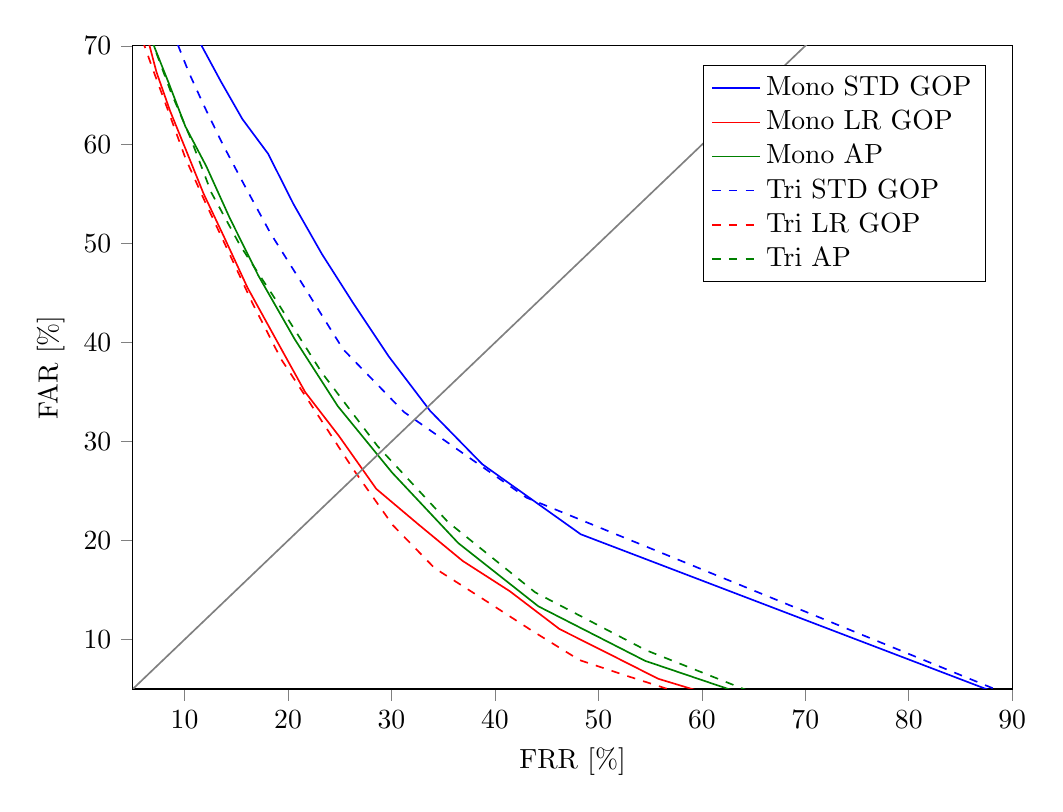
\begin{tikzpicture}

\begin{axis}[
tick align=outside,
tick pos=left,
x grid style={white!69.01960784313725!black},
xlabel={FRR [\%]},
xmin=5, xmax=90,
y grid style={white!69.01960784313725!black},
ylabel={FAR [\%]},
ymin=5, ymax=70,
legend pos=north east,
width=12.75cm,
height=9.75cm,
legend cell align={left},
]

\addplot [semithick, blue]
table {%
100 0
48.295262743333 20.6355591311344
38.7794906417614 27.7152051488335
33.7384194141255 33.1053901850362
29.7588237500469 38.5760257441673
26.2443269194704 44.0868865647627
23.2774464573722 48.9541432019308
20.5393646149807 53.9823008849557
18.0750909568283 59.0909090909091
15.5920633134541 62.5905068382944
13.5028693597389 66.4119066773934
11.5712088818874 70.152855993564
9.80083267694385 73.9742558326629
8.47680132028056 77.1118262268705
7.18652713701662 80.1287208366854
6.03503244439443 82.4215607401448
5.00731405423653 84.3523732904264
4.11462435767601 85.880933226066
3.37196654289036 87.5703942075624
2.76058662465774 89.0185036202735
2.28048460297813 90.2654867256637
1.8566445369641 91.2308930008045
1.52657439705938 91.9147224456959
1.23776302464274 92.8399034593725
1.02021679606916 93.3628318584071
0.8551817261168 94.2075623491553
0.697648250253179 94.8109412711183
0.573871947788905 95.3740949316171
0.468849630546491 96.0176991150443
0.363827313304077 96.2590506838295
0.296312966505382 96.7417538213998
0.262555793106035 97.3451327433628
0.225047822662316 97.6267095736122
0.202543040396084 97.98873692679
0.191290649262968 98.2300884955752
0.180038258129853 98.592115848753
0.161284272907993 98.8736926790024
0.131277896553018 98.994368463395
0.108773114286786 99.0748189863234
0.0975207231536701 99.1552695092518
0.0900191290649263 99.2759452936444
0.0787667379318105 99.4368463395012
0.0750159408874386 99.597747385358
0.0562619556655789 99.597747385358
0.0412587674880912 99.597747385358
0.0337571733993474 99.597747385358
0.0300063763549754 99.7184231697506
0.0300063763549754 99.7586484312148
0.0262555793106035 99.798873692679
0.0262555793106035 99.8390989541432
0.0187539852218596 99.9597747385358
0.0187539852218596 100
0.0150031881774877 100
0.0112523911331158 100
0.00750159408874386 100
0.00375079704437193 100
}; \addlegendentry{Mono STD GOP}

\addplot [semithick, red]
table {%
0.00375079704437193 100
0.00750159408874386 100
0.0112523911331158 100
0.0150031881774877 100
0.0187539852218596 100
0.0225047822662316 100
0.0225047822662316 99.8793242156074
0.0262555793106035 99.798873692679
0.0262555793106035 99.798873692679
0.0300063763549754 99.7586484312148
0.0300063763549754 99.6781979082864
0.0412587674880912 99.597747385358
0.0487603615768351 99.4770716009654
0.0600127527099509 99.396621078037
0.0787667379318105 99.3563958165728
0.0825175349761824 99.1552695092518
0.101271520198042 98.994368463395
0.105022317242414 98.793242156074
0.11627470837553 98.7530168946098
0.135028693597389 98.5116653258246
0.165035069952365 98.3507642799678
0.180038258129853 97.98873692679
0.202543040396084 97.8680611423974
0.221297025617944 97.6669348350764
0.243801807884175 97.2646822204344
0.285060575372267 96.8222043443282
0.33007013990473 96.2590506838295
0.367578110348449 95.6958970233307
0.4275908630584 95.4143201930813
0.528862383256442 94.7707160096541
0.615130715276996 94.0064360418343
0.716402235475038 93.4030571198713
0.810172161584337 92.6387771520515
0.941450058137354 91.8342719227675
1.10273433104535 90.5872888173773
1.3090281684858 89.8632341110217
1.50782041183752 88.7771520514883
1.75162221972169 87.4497184231698
2.07794156258205 85.9613837489944
2.41926409361989 84.5534995977474
2.90686770938825 83.1858407079646
3.45448407786655 80.9734513274336
4.04711001087731 79.444891391794
4.67349311728742 76.6291230893001
5.47241288773864 74.0144810941271
6.36510258429916 70.9975864843122
7.28779865721466 67.33708769107
8.60807921683358 63.3950120675784
10.1271520198042 59.4931617055511
11.8337646749934 55.0683829444891
13.9079554405311 50.4827031375704
16.0759161321781 45.575221238938
18.7652376129928 40.4666130329847
21.6608529312479 34.9959774738536
24.9202955628071 30.5711987127916
28.5323131165373 25.2212389380531
32.5944263155921 21.6411906677393
36.8853381343536 17.940466613033
41.4350549491767 14.8833467417538
46.2360751659728 11.0619469026549
50.988335021192 8.5679806918745
55.7818536438993 6.03378921962993
60.2227973444357 4.62590506838295
64.4686995986647 3.41914722445696
68.4820524361427 2.77554304102977
72.1503319455384 1.85036202735318
75.6235700086268 1.32743362831858
78.4741757623495 0.764279967819791
81.3885450658265 0.482703137570394
84.2053936461498 0.402252614641995
86.5308878136604 0.241351568785197
88.6500881437305 0.120675784392599
90.3454484077866 0.080450522928399
91.9207831664229 0.080450522928399
93.1472937999325 0.0402252614641995
94.201267769401 0.0402252614641995
95.1614718127602 0
95.8403660777915 0
96.5567683132666 0
97.1343910580999 0
97.6182438768238 0
98.1358538689472 0
98.5146843704287 0
98.8785116837328 0
99.1410674768388 0
99.2873485615693 0
99.4223772551667 0
99.5799107310303 0
99.6849330482728 0
99.7899553655152 0
99.8799744945801 0
99.9062300738907 0
99.9137316679794 0
99.9549904354675 0
99.9737444206894 0
99.9774952177338 0
99.9849968118225 0
99.9887476088669 0
100 0
}; \addlegendentry{Mono LR GOP}

\addplot [semithick, green!50!black]
table {%
0 100
0.00375079704437193 100
0.00750159408874386 100
0.0112523911331158 100
0.0150031881774877 100
0.0187539852218596 100
0.0225047822662316 99.9597747385358
0.0262555793106035 99.9597747385358
0.0300063763549754 99.8793242156074
0.0337571733993474 99.8390989541432
0.0375079704437193 99.8390989541432
0.0450095645324631 99.8390989541432
0.0562619556655789 99.7184231697506
0.0675143467986947 99.6379726468222
0.0712651438430666 99.5172968624296
0.0750159408874386 99.4368463395012
0.0900191290649263 99.3563958165728
0.0975207231536701 99.1150442477876
0.11627470837553 98.9541432019308
0.127527099508646 98.8334674175382
0.146281084730505 98.7127916331456
0.157533475863621 98.592115848753
0.183789055174225 98.390989541432
0.19504144630734 98.3105390185036
0.221297025617944 97.98873692679
0.243801807884175 97.7473853580048
0.288811372416639 97.3049074818986
0.315066951727242 96.983105390185
0.360076516259705 96.5406275140788
0.382581298525937 96.2590506838295
0.453846442369003 95.6556717618665
0.540114774389558 95.1327433628319
0.600127527099509 94.5695897023331
0.693897453208807 93.7650844730491
0.806421364539965 92.9203539823009
0.922696072915495 91.9951729686243
1.14024230148907 90.9090909090909
1.30527737144143 90.0643604183427
1.54907917932561 89.0989541432019
1.8041333783429 87.8519710378118
2.14545590938074 86.3234111021722
2.50553242564045 84.2316975060338
2.97063125914257 82.5824617860016
3.54450320693147 80.65164923572
4.17838790743033 78.4794851166533
4.93979970743783 76.0659694288013
5.94501331532951 73.4513274336283
7.10025880499606 69.8310539018504
8.46554892914744 66.2510056315366
10.0708900641386 61.8664521319389
12.0925696710551 57.8439259855189
14.3768050710776 52.5744167337088
17.1298901016466 46.781979082864
20.6481377292675 40.3459372485921
24.8077716514759 33.5880933226066
30.0588875135966 26.8704746580853
36.4502456772064 19.750603378922
44.1993923708788 13.3547868061142
54.5215858369904 7.84392598551891
68.5045572184089 2.89621882542237
88.3312703949589 0.362027353177796
100 0
}; \addlegendentry{Mono AP}

\addplot [semithick, dashed, blue]
table {%
100 0
43.0478976782566 24.3362831858407
31.2141330032632 32.9847144006436
25.3178800495105 39.3403057119871
21.3345335883875 46.0176991150442
18.2888863883575 51.0860820595334
15.7833539627171 55.9131134352373
13.7016616030907 60.0160901045857
11.890026630659 63.917940466613
10.4009602040434 67.33708769107
9.08818123851318 70.7964601769911
7.96294212520161 73.8133547868061
6.95772851730993 76.4279967819791
6.1062975882375 78.9219629927594
5.29987622369754 81.6170555108608
4.61723116162184 83.9501206757844
3.9945988522561 86.1625100563154
3.50699523648775 87.3692679002414
2.9931360414088 88.9782783588093
2.64056111923784 90.5068382944489
2.24672742957879 91.4722445695897
1.86039533400848 92.5181013676589
1.54157758523686 93.5237329042639
1.24151382168711 94.5293644408689
0.978958028581074 95.4545454545455
0.8551817261168 96.1383748994369
0.667641873898203 96.5004022526146
0.54386557143393 97.184231697506
0.44634484828026 97.787610619469
0.326319342860358 97.98873692679
0.277558981283523 98.390989541432
0.221297025617944 98.4714400643604
0.165035069952365 98.7530168946098
0.142530287686133 98.8736926790024
0.11627470837553 99.0748189863234
0.0900191290649263 99.195494770716
0.0825175349761824 99.2759452936444
0.0675143467986947 99.4770716009654
0.0412587674880912 99.5172968624296
0.0337571733993474 99.5172968624296
0.0262555793106035 99.597747385358
0.0225047822662316 99.6379726468222
0.0225047822662316 99.7184231697506
0.0187539852218596 99.7586484312148
0.0187539852218596 99.7586484312148
0.0187539852218596 99.798873692679
0.0187539852218596 99.9195494770716
0.0187539852218596 99.9195494770716
0.0187539852218596 99.9195494770716
0.0112523911331158 99.9195494770716
0.0112523911331158 99.9195494770716
0.0112523911331158 99.9195494770716
0.0112523911331158 99.9597747385358
0.0112523911331158 99.9597747385358
0.0112523911331158 99.9597747385358
0.00750159408874386 99.9597747385358
0.00750159408874386 99.9597747385358
0.00750159408874386 99.9597747385358
0.00750159408874386 99.9597747385358
0.00375079704437193 99.9597747385358
0.00375079704437193 99.9597747385358
0.00375079704437193 99.9597747385358
0.00375079704437193 100
0.00375079704437193 100
0.00375079704437193 100
0 100
}; \addlegendentry{Tri STD GOP}

\addplot [semithick, dashed, red]
table {%
0 100
0.00375079704437193 100
0.00750159408874386 99.9597747385358
0.0112523911331158 99.9597747385358
0.0112523911331158 99.9597747385358
0.0112523911331158 99.9195494770716
0.0112523911331158 99.9195494770716
0.0112523911331158 99.9195494770716
0.0112523911331158 99.9195494770716
0.0187539852218596 99.9195494770716
0.0187539852218596 99.9195494770716
0.0187539852218596 99.9195494770716
0.0187539852218596 99.798873692679
0.0187539852218596 99.7586484312148
0.0187539852218596 99.7586484312148
0.0300063763549754 99.6781979082864
0.0300063763549754 99.597747385358
0.0412587674880912 99.5575221238938
0.0487603615768351 99.4368463395012
0.0562619556655789 99.4368463395012
0.0675143467986947 99.396621078037
0.0787667379318105 99.195494770716
0.0825175349761824 99.1552695092518
0.0825175349761824 98.994368463395
0.0975207231536701 98.6725663716814
0.11627470837553 98.4714400643604
0.135028693597389 98.1094127111826
0.168785866996737 97.8680611423974
0.180038258129853 97.6669348350764
0.210044634484828 97.184231697506
0.273808184239151 96.7015285599356
0.307565357638498 95.9372485921158
0.341322531037846 95.5349959774739
0.393833689659053 95.0120675784393
0.476351224635235 94.3684633950121
0.588875135966393 93.6041834271923
0.686395859120063 92.6387771520515
0.825175349761824 91.5929203539823
1.01271520198042 90.6677393403057
1.21900903942088 89.5012067578439
1.48156483252691 87.6508447304907
1.77412700198792 86.0016090104586
2.18671467686883 84.3121480289622
2.67806908968156 82.260659694288
3.26694422564795 79.8069187449718
3.95334008476801 77.1118262268705
4.87978695472788 74.0547063555913
5.8925021567083 70.6757843925985
7.09275721090732 67.1761866452132
8.4580473350587 63.31456154465
10.0821424552717 58.6484312148029
11.860020254304 54.5052292839903
14.1517572484153 49.396621078037
16.5935261243014 43.9259855189059
19.3541127489592 38.2944489139179
22.6698173361839 33.0249396621078
26.3418476426241 27.1520514883347
30.1264018603953 21.5607401448109
34.1660102771839 17.2164119066774
38.9332733205806 14.0386162510056
43.56550767038 10.9010458567981
48.1714864408687 7.9243765084473
53.0212670192416 6.23491552695093
57.9310603503245 4.58567980691874
62.7020741907655 3.09734513274336
66.9404748509058 2.13193885760257
71.0400960204043 1.52855993563958
74.9859345110836 1.04585679806919
78.6767188027456 0.884955752212389
81.9624170136154 0.563153660498793
84.8617831289149 0.362027353177796
87.333558381156 0.241351568785197
89.5277746521136 0.241351568785197
91.3206556393234 0.160901045856798
92.9109935861371 0.120675784392599
94.3700536363977 0.120675784392599
95.4015228236 0.0402252614641995
96.2904617231162 0.0402252614641995
97.145643449233 0
97.8057837290424 0
98.2783841566333 0
98.7584861783129 0
99.0435467536852 0
99.2986009527025 0
99.4523836315217 0
99.5836615280747 0
99.7186902216721 0
99.8049585536927 0
99.8649713064026 0
99.9062300738907 0
99.93998724729 0
99.9624920295563 0
99.9812460147781 0
99.9924984059113 0
99.9962492029556 0
100 0
}; \addlegendentry{Tri LR GOP}

\addplot [semithick, dashed, green!50!black]
table {%
0 100
0.00375079704437193 100
0.00375079704437193 99.9597747385358
0.00375079704437193 99.9195494770716
0.00750159408874386 99.9195494770716
0.0112523911331158 99.8793242156074
0.0112523911331158 99.8793242156074
0.0112523911331158 99.8793242156074
0.0150031881774877 99.8793242156074
0.0225047822662316 99.8390989541432
0.0225047822662316 99.7586484312148
0.0262555793106035 99.7184231697506
0.0300063763549754 99.7184231697506
0.0337571733993474 99.7184231697506
0.0375079704437193 99.6379726468222
0.0487603615768351 99.6379726468222
0.052511158621207 99.5575221238938
0.0562619556655789 99.4368463395012
0.0562619556655789 99.3161705551086
0.0750159408874386 99.1552695092518
0.0825175349761824 98.8334674175382
0.101271520198042 98.793242156074
0.11627470837553 98.5116653258246
0.138779490641761 98.189863234111
0.180038258129853 97.787610619469
0.221297025617944 97.586484312148
0.243801807884175 97.2646822204344
0.270057387194779 96.8222043443282
0.296312966505382 96.5004022526146
0.326319342860358 96.0176991150443
0.397584486703425 95.3338696701529
0.472600427590863 94.5293644408689
0.551367165522674 94.0466613032985
0.697648250253179 93.1214802896219
0.851430929072428 92.1962992759453
0.97145643449233 91.0297666934835
1.15899628671093 89.9034593724859
1.41029968868385 88.5358004827031
1.67660627883425 87.0072405470636
2.02167960691647 85.1166532582462
2.53178800495105 82.9444891391794
3.04939799707438 80.7723250201126
3.79205581186002 78.5197103781175
4.66599152319868 75.9050683829445
5.83248940399835 73.1295253419147
7.19027793406099 69.5092518101368
8.67934436067664 65.32582461786
10.6147556355726 60.5792437650845
12.5951764750009 55.1488334674175
15.4045234612355 49.7586484312148
18.9415250740782 44.1271118262269
23.2699448632834 36.9670152855994
28.6373354337797 29.5655671761866
35.4525336634035 21.8825422365245
43.8955778102847 14.7626709573612
54.5815985897003 8.93000804505229
68.7221034469825 3.05711987127916
88.7438580698398 0.522928399034594
100 0
}; \addlegendentry{Tri AP}

\addplot [semithick, gray, forget plot]
table [row sep=\\]{%
0	0 \\
0.50251256281407	0.50251256281407 \\
1.00502512562814	1.00502512562814 \\
1.50753768844221	1.50753768844221 \\
2.01005025125628	2.01005025125628 \\
2.51256281407035	2.51256281407035 \\
3.01507537688442	3.01507537688442 \\
3.51758793969849	3.51758793969849 \\
4.02010050251256	4.02010050251256 \\
4.52261306532663	4.52261306532663 \\
5.0251256281407	5.0251256281407 \\
5.52763819095477	5.52763819095477 \\
6.03015075376884	6.03015075376884 \\
6.53266331658291	6.53266331658291 \\
7.03517587939698	7.03517587939698 \\
7.53768844221105	7.53768844221105 \\
8.04020100502512	8.04020100502512 \\
8.5427135678392	8.5427135678392 \\
9.04522613065327	9.04522613065327 \\
9.54773869346734	9.54773869346734 \\
10.0502512562814	10.0502512562814 \\
10.5527638190955	10.5527638190955 \\
11.0552763819095	11.0552763819095 \\
11.5577889447236	11.5577889447236 \\
12.0603015075377	12.0603015075377 \\
12.5628140703518	12.5628140703518 \\
13.0653266331658	13.0653266331658 \\
13.5678391959799	13.5678391959799 \\
14.070351758794	14.070351758794 \\
14.572864321608	14.572864321608 \\
15.0753768844221	15.0753768844221 \\
15.5778894472362	15.5778894472362 \\
16.0804020100502	16.0804020100502 \\
16.5829145728643	16.5829145728643 \\
17.0854271356784	17.0854271356784 \\
17.5879396984925	17.5879396984925 \\
18.0904522613065	18.0904522613065 \\
18.5929648241206	18.5929648241206 \\
19.0954773869347	19.0954773869347 \\
19.5979899497487	19.5979899497487 \\
20.1005025125628	20.1005025125628 \\
20.6030150753769	20.6030150753769 \\
21.105527638191	21.105527638191 \\
21.608040201005	21.608040201005 \\
22.1105527638191	22.1105527638191 \\
22.6130653266332	22.6130653266332 \\
23.1155778894472	23.1155778894472 \\
23.6180904522613	23.6180904522613 \\
24.1206030150754	24.1206030150754 \\
24.6231155778894	24.6231155778894 \\
25.1256281407035	25.1256281407035 \\
25.6281407035176	25.6281407035176 \\
26.1306532663317	26.1306532663317 \\
26.6331658291457	26.6331658291457 \\
27.1356783919598	27.1356783919598 \\
27.6381909547739	27.6381909547739 \\
28.1407035175879	28.1407035175879 \\
28.643216080402	28.643216080402 \\
29.1457286432161	29.1457286432161 \\
29.6482412060301	29.6482412060301 \\
30.1507537688442	30.1507537688442 \\
30.6532663316583	30.6532663316583 \\
31.1557788944724	31.1557788944724 \\
31.6582914572864	31.6582914572864 \\
32.1608040201005	32.1608040201005 \\
32.6633165829146	32.6633165829146 \\
33.1658291457286	33.1658291457286 \\
33.6683417085427	33.6683417085427 \\
34.1708542713568	34.1708542713568 \\
34.6733668341708	34.6733668341708 \\
35.1758793969849	35.1758793969849 \\
35.678391959799	35.678391959799 \\
36.1809045226131	36.1809045226131 \\
36.6834170854271	36.6834170854271 \\
37.1859296482412	37.1859296482412 \\
37.6884422110553	37.6884422110553 \\
38.1909547738693	38.1909547738693 \\
38.6934673366834	38.6934673366834 \\
39.1959798994975	39.1959798994975 \\
39.6984924623116	39.6984924623116 \\
40.2010050251256	40.2010050251256 \\
40.7035175879397	40.7035175879397 \\
41.2060301507538	41.2060301507538 \\
41.7085427135678	41.7085427135678 \\
42.2110552763819	42.2110552763819 \\
42.713567839196	42.713567839196 \\
43.21608040201	43.21608040201 \\
43.7185929648241	43.7185929648241 \\
44.2211055276382	44.2211055276382 \\
44.7236180904523	44.7236180904523 \\
45.2261306532663	45.2261306532663 \\
45.7286432160804	45.7286432160804 \\
46.2311557788945	46.2311557788945 \\
46.7336683417085	46.7336683417085 \\
47.2361809045226	47.2361809045226 \\
47.7386934673367	47.7386934673367 \\
48.2412060301507	48.2412060301507 \\
48.7437185929648	48.7437185929648 \\
49.2462311557789	49.2462311557789 \\
49.748743718593	49.748743718593 \\
50.251256281407	50.251256281407 \\
50.7537688442211	50.7537688442211 \\
51.2562814070352	51.2562814070352 \\
51.7587939698492	51.7587939698492 \\
52.2613065326633	52.2613065326633 \\
52.7638190954774	52.7638190954774 \\
53.2663316582914	53.2663316582914 \\
53.7688442211055	53.7688442211055 \\
54.2713567839196	54.2713567839196 \\
54.7738693467337	54.7738693467337 \\
55.2763819095477	55.2763819095477 \\
55.7788944723618	55.7788944723618 \\
56.2814070351759	56.2814070351759 \\
56.7839195979899	56.7839195979899 \\
57.286432160804	57.286432160804 \\
57.7889447236181	57.7889447236181 \\
58.2914572864322	58.2914572864322 \\
58.7939698492462	58.7939698492462 \\
59.2964824120603	59.2964824120603 \\
59.7989949748744	59.7989949748744 \\
60.3015075376884	60.3015075376884 \\
60.8040201005025	60.8040201005025 \\
61.3065326633166	61.3065326633166 \\
61.8090452261306	61.8090452261306 \\
62.3115577889447	62.3115577889447 \\
62.8140703517588	62.8140703517588 \\
63.3165829145729	63.3165829145729 \\
63.8190954773869	63.8190954773869 \\
64.321608040201	64.321608040201 \\
64.8241206030151	64.8241206030151 \\
65.3266331658291	65.3266331658291 \\
65.8291457286432	65.8291457286432 \\
66.3316582914573	66.3316582914573 \\
66.8341708542713	66.8341708542713 \\
67.3366834170854	67.3366834170854 \\
67.8391959798995	67.8391959798995 \\
68.3417085427136	68.3417085427136 \\
68.8442211055276	68.8442211055276 \\
69.3467336683417	69.3467336683417 \\
69.8492462311558	69.8492462311558 \\
70.3517587939699	70.3517587939699 \\
70.8542713567839	70.8542713567839 \\
71.356783919598	71.356783919598 \\
71.859296482412	71.859296482412 \\
72.3618090452261	72.3618090452261 \\
72.8643216080402	72.8643216080402 \\
73.3668341708543	73.3668341708543 \\
73.8693467336683	73.8693467336683 \\
74.3718592964824	74.3718592964824 \\
74.8743718592965	74.8743718592965 \\
75.3768844221105	75.3768844221105 \\
75.8793969849246	75.8793969849246 \\
76.3819095477387	76.3819095477387 \\
76.8844221105528	76.8844221105528 \\
77.3869346733668	77.3869346733668 \\
77.8894472361809	77.8894472361809 \\
78.391959798995	78.391959798995 \\
78.894472361809	78.894472361809 \\
79.3969849246231	79.3969849246231 \\
79.8994974874372	79.8994974874372 \\
80.4020100502512	80.4020100502512 \\
80.9045226130653	80.9045226130653 \\
81.4070351758794	81.4070351758794 \\
81.9095477386935	81.9095477386935 \\
82.4120603015075	82.4120603015075 \\
82.9145728643216	82.9145728643216 \\
83.4170854271357	83.4170854271357 \\
83.9195979899497	83.9195979899497 \\
84.4221105527638	84.4221105527638 \\
84.9246231155779	84.9246231155779 \\
85.4271356783919	85.4271356783919 \\
85.929648241206	85.929648241206 \\
86.4321608040201	86.4321608040201 \\
86.9346733668342	86.9346733668342 \\
87.4371859296482	87.4371859296482 \\
87.9396984924623	87.9396984924623 \\
88.4422110552764	88.4422110552764 \\
88.9447236180904	88.9447236180904 \\
89.4472361809045	89.4472361809045 \\
89.9497487437186	89.9497487437186 \\
90.4522613065326	90.4522613065326 \\
90.9547738693467	90.9547738693467 \\
91.4572864321608	91.4572864321608 \\
91.9597989949749	91.9597989949749 \\
92.4623115577889	92.4623115577889 \\
92.964824120603	92.964824120603 \\
93.4673366834171	93.4673366834171 \\
93.9698492462311	93.9698492462311 \\
94.4723618090452	94.4723618090452 \\
94.9748743718593	94.9748743718593 \\
95.4773869346734	95.4773869346734 \\
95.9798994974874	95.9798994974874 \\
96.4824120603015	96.4824120603015 \\
96.9849246231156	96.9849246231156 \\
97.4874371859296	97.4874371859296 \\
97.9899497487437	97.9899497487437 \\
98.4924623115578	98.4924623115578 \\
98.9949748743718	98.9949748743718 \\
99.4974874371859	99.4974874371859 \\
100	100 \\
};

\end{axis}

\end{tikzpicture}
    \caption{Graf závislosti FAR a FRR pre metódy založené na aposteriórnej pravdepodobnosti foném -- štandardné GOP (STD GOP), likelihood-ratio GOP (LR GOP) a spriemerované aposteriórne pravdepodobnosti (AP).} \label{fig:roc-gop-methods}
\end{figure}

\begin{table}[h!]
\centering
\begin{tabular}{@{}llll@{}}
\toprule
EER {[}\%{]} & STD GOP & LR GOP  & AP \\ \midrule
Mono AM      & $33{,}35$   & $\bm{27{,}23}$   & $28{,}60$  \\
Tri AM       & $31{,}74$   & $\bm{26{,}91}$   & $29{,}00$  \\ \bottomrule
\end{tabular}
\caption{Výsledky dosiahnuté pomocou štandardnej GOP metódy (STD GOP), modifikácie založenej na počítaní pomeru vierohodností (LR GOP) a spriemerovanými aposteriórnými pravdepodobnostiami (AP).} \label{tab:eer-gop-methods}
\end{table} 

\section{Porovnanie metód založených na priamej klasifikácii}

Obdobným spôsobom porovnáme rôzne metódy založené na priamej klasifikácii. Okrem dopredných neurónových sietí využívajúcich ako príznaky vierohodnosti HMM stavov (NN HMM) a pravdepobnosti fonologických rysov (NN PFeats) sa zameriame aj na použitie LSTM neurónových sietí nad rovnakými príznakmi (LSTM HMM, resp. LSTM PFeats). Pri klasifikátoroch pracujúcich s~fonologickými rysmi využijeme len monofónový akustický model, nakoľko v~tomto prípade slúži len na získanie nútených zarovnaní, ktoré sú pri trifónovom modeli takmer totožné.

Pri klasifikácii pomocou LSTM je možné očakávať mierne lepšie výsledky, nakoľko takáto neurónová sieť pracuje so všetkými rámcami daného segmentu. V~prípade jednoduchej neurónovej siete je totiž tieto príznaky nutné spriemerovať, čím môže dôjsť k~strate dôležitej informácie o~kontexte.

Už pri prvom pohľade na graf \ref{fig:roc-classifiers} je vidieť, že klasifikátory pracujúce s~vierohodnosťami HMM stavov dosahujú nezanedbateľne lepšie výsledky ako je tomu pri klasifikátoroch založených na pravdepodobnostiach fonologických rysov. EER medzi NN HMM a NN PFeats metódami sa líši o~$0{,}92$ percentuálnych bodov, čo predstavuje zlepšenie o~$3{,}2\,\%$ pri NN HMM klasifikátore. Takýto záver však nie je veľkým prekvapením. V~prvom rade totiž vierohodností HMM stavov majú značne väčšiu dimenziu (150 vs. 19), takže sa dá očakávať, že nesú aj viacej informácie. Okrem toho sa môže veľké množstvo informácie stratiť už pri trénovaní neurónovej siete určujúcej fonologické rysy. Pri ňom sa totiž fonologické rysy stanovujú pomocou tabuľky prevodom z~fonémového prepisu. Takýto prevod ale môže zaniesť do trénovania veľa chýb daných variabilitou reči. Napokon takýto prevod je len lineárnou funkciou, ktorú sa môže naučiť aj samotná neurónová sieť stanovujúca HMM stavy. To dokazuje aj práca od Nagamine a kol. \cite{Nagamine2015}, ktorá vizuálizáciou ukázala, že v~skrytých vrstvách DNN akustického modelu sa formujú skupiny neurónov, ktoré pripomínajú fonologické rysy.

Očakávané zlepšenie sme pri použití LSTM nedosiahli. Pri oboch druhoch príznakov tento typ klasifikátora vykázal horšie výsledky ako jednoduchá neurónová sieť. Najmä v~prípade fonologických rysov bola EER o~$1{,}8$ percentuálnych bodov vyššia než pri jednoduchej neurónovej sieti, čo znamená relatívne zhoršenie o~$6{,}32\,\%$. Príčinou je zrejme nepomer v~počte parametrov LSTM modelu a veľkosti trénovacej sady. V~porovnaní s~jednoduchou neurónovou sieťou je totiž počet parametrov násobne vyšší (406\,058 vs. 44\,074 pri monofónovom AM, 2\,215\,466 vs. 496\,426 pri trifónovom AM). 

\begin{table}[h!]
    \centering
    \begin{tabular}{@{}lllll@{}}
    \toprule
    EER {[}\%{]} & NN HMM        & LSTM HMM & NN PFeats          & LSTM PFeats \\ \midrule
    Mono AM      & $\bm{27{,}57} \pm 0{,}16$ & $27{,}99 \pm 0{,}24$  & $28{,}49 \pm 0{,}14$      & $30{,}29 \pm 0{,}10$           \\
    Tri AM       & $\bm{27{,}06} \pm 0{,}18$ & $28{,}00 \pm 0{,}12$        & -       & -           \\ \bottomrule
    \end{tabular}
    \label{tab:eer-classifiers}
    \caption{Výsledky dosiahnuté metódami založenými na priamej klasifikácii pomocou neurónových sietí (NN), resp. LSTM neurónových sietí, ktoré boli trénované na vierohodnostiach HMM stavov (NN HMM, resp. LSTM HMM), a na pravdepodobnostiach fonologických rysov (NN PFeats, resp. LSTM PFeats).}
\end{table}

\begin{figure}[h!]
    \centering
    % This file was created by matplotlib2tikz v0.6.18.
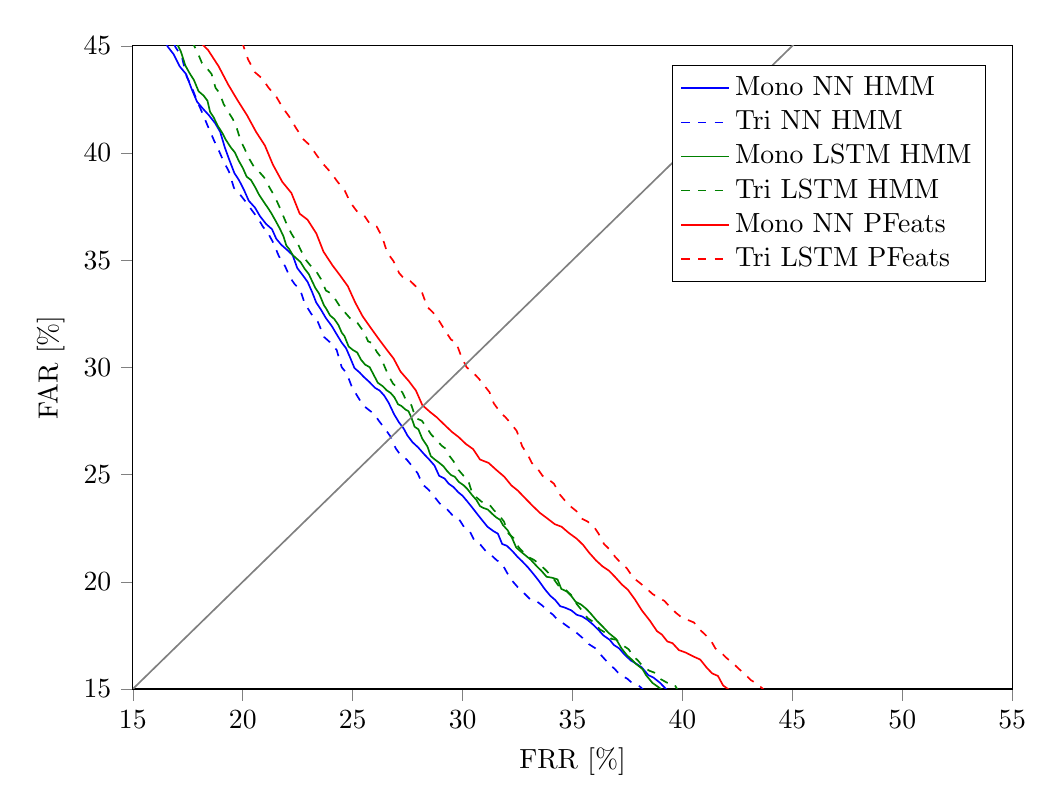
\begin{tikzpicture}

\begin{axis}[
tick align=outside,
tick pos=left,
x grid style={white!69.01960784313725!black},
xlabel={FRR [\%]},
xmin=15, xmax=55,
y grid style={white!69.01960784313725!black},
ylabel={FAR [\%]},
ymin=15, ymax=45,
legend pos=north east,
width=12.75cm,
height=9.75cm,
legend cell align={left},
]

\addplot [semithick, blue]
table {%
0 100
2.50928322268482 85.2373290426388
3.66827950939575 81.2148028962188
4.66974232024305 77.1922767497989
5.3711413675406 74.8994368463395
5.92625933010765 72.3250201126307
6.58264881287274 70.3942075623492
7.11151119612918 68.946098149638
7.61411800007502 67.4979887369268
8.04170886313342 66.5728077232502
8.50305689959116 64.8028962188254
8.87063500993961 63.1938857602574
9.32823224935299 62.0273531777957
9.79333108285511 61.2228479485117
10.2171711488691 59.9758648431215
10.5734968680845 59.2518101367659
10.9860845429654 57.9646017699115
11.3011514946926 56.9589702333065
11.6499756198192 56.1946902654867
11.9987997449458 55.2292839903459
12.3363714789393 54.5052292839903
12.6626908217996 53.9018503620273
13.0077641498819 53.1777956556718
13.3190803045647 52.3330651649236
13.6566520385582 51.6492357200322
13.9379618168861 51.1263073209976
14.2680319567908 50.4827031375704
14.54184014103 49.8793242156074
14.7706387607367 49.1552695092518
15.0181913656652 48.6323411102172
15.2957503469487 47.9485116653258
15.5583061400548 47.4658085277554
15.7570983834065 46.8624296057924
16.0009001912906 46.1383748994368
16.2709575784854 45.776347546259
16.5785229361239 44.9718423169751
16.8523311203631 44.6098149637973
17.1261393046022 44.0466613032985
17.4187014740632 43.6846339501207
17.6850080642136 42.9605792437651
17.9175574809647 42.3974255832663
18.1801132740707 42.0756234915527
18.465173849443 41.7538213998391
18.7427328307265 41.3917940466613
18.9715314504332 40.9895414320193
19.181576084918 40.2654867256637
19.3503619519148 39.7827835880933
19.6204193391096 39.0587288817377
19.82671317655 38.7369267900241
20.048010202168 38.2944489139179
20.2730580248303 37.7715205148833
20.5581186002025 37.4497184231698
20.7869172199092 37.0474658085278
21.0644762011928 36.68543845535
21.3307827913432 36.4440868865648
21.5220734406061 36.0016090104586
21.7508720603128 35.7200321802092
22.0171786504632 35.478680611424
22.2684820524361 35.2373290426388
22.478526686921 34.6339501206758
22.7485840741157 34.271922767498
22.9473763174675 33.9903459372486
23.1574209519523 33.5076427996782
23.3412100071265 33.0249396621078
23.5512546416113 32.7031375703942
23.780053261318 32.3008849557522
24.0426090544241 31.9388576025744
24.2526536889089 31.5768302493966
24.4889539027043 31.1745776347546
24.6989985371892 30.8930008045052
24.8865383894078 30.450522928399
25.0815798357151 29.9678197908286
25.3103784554218 29.7666934835076
25.494167510596 29.5655671761866
25.7529725066577 29.3242156074014
26.0192790968081 29.0426387771521
26.2255729342485 28.9219629927595
26.4356175687334 28.6806114239743
26.6306590150407 28.3588093322607
26.8932148081467 27.7956556717619
27.1070102396759 27.4336283185841
27.3170548741608 27.1520514883347
27.4858407411575 26.8302493966211
27.7221409549529 26.5084473049075
27.9771951539702 26.2670957361223
28.2547541352537 25.9452936444087
28.4798019579161 25.7039420756235
28.7198529687559 25.4223652453741
28.9336484002851 24.9396621078037
29.1774502081692 24.8189863234111
29.3649900603878 24.5776347546259
29.5862870860058 24.4167337087691
29.8038333145793 24.1753821399839
29.9951239638423 24.0144810941271
30.193916207194 23.7731295253419
30.415213232812 23.4915526950925
30.6590150406961 23.1697506033789
30.8765612692697 22.8881737731295
31.131615468287 22.5663716814159
31.3979220584374 22.3652453740949
31.6042158958779 22.2445695897023
31.7992573421852 21.7618664521319
32.00930197667 21.6814159292035
32.2568545815986 21.4400643604183
32.5006563894828 21.1584875301689
32.7069502269232 20.9573612228479
32.9695060200293 20.6757843925986
33.2620681894903 20.3137570394208
33.4758636210195 20.0321802091714
33.7271670229924 19.6701528559936
33.9859720190541 19.34835076428
34.2147706387607 19.147224456959
34.4360676643787 18.8656476267096
34.6761186752185 18.7851971037812
34.9499268594576 18.6645213193886
35.1862270732531 18.4633950120676
35.437530475226 18.3829444891392
35.6850830801545 18.2220434432824
35.9138816998612 18.0209171359614
36.1576835077454 17.7795655671762
36.4052361126739 17.4979887369268
36.6865458910018 17.2968624296058
36.8778365402648 17.0555108608206
37.1178875511046 16.8946098149638
37.3579385619444 16.6130329847144
37.6467499343611 16.331456154465
37.9130565245115 16.1705551086082
38.1456059412625 16.0096540627514
38.4456697048123 15.6476267095736
38.6857207156521 15.526950925181
38.9820336821575 15.2855993563958
39.2483402723079 15.0040225261464
39.582161209257 14.722445695897
39.8709725816736 14.6017699115044
40.1410299688684 14.3604183427192
40.4073365590188 14.0386162510056
40.7411574959679 13.7972646822204
41.044972056562 13.5961383748994
41.337534226023 13.3950120675784
41.630096395484 13.2341110217216
41.9376617531225 12.8720836685438
42.2114699373617 12.6307320997586
42.5040321068227 12.4698310539019
42.7515847117512 12.1882542236525
43.0929072427891 11.9066773934031
43.4679869472263 11.7860016090105
43.7943062900866 11.5848753016895
44.1581336033907 11.4239742558327
44.5144593226061 11.2228479485117
44.8520310565995 11.0619469026549
45.1783503994599 10.8608205953339
45.5084205393646 10.4987932421561
45.9435129965118 10.0965406275141
46.3298450920821 9.65406275140788
46.6936724053861 9.33226065969429
47.0987584861783 9.17135961383749
47.4550842053936 8.84955752212389
47.8564194891414 8.6484312148029
48.2877611492442 8.4875301689461
48.6665916507258 8.2461786001609
49.1016841078729 8.0048270313757
49.5030193916207 7.9243765084473
49.8330895315254 7.68302493966211
50.2681819886726 7.48189863234111
50.6845204605979 7.20032180209171
51.1608716852331 6.87851971037812
51.603465736469 6.63716814159292
52.0948201492817 6.51649235720032
52.6274333295825 6.31536604987932
53.1675481039721 6.15446500402253
53.6926596901842 5.95333869670153
54.2290236675294 5.63153660498793
54.6978732980758 5.18905872888174
55.2717452458647 4.98793242156074
55.8906267581861 4.82703137570394
56.4982558793744 4.58567980691874
57.1846517384944 4.34432823813355
57.9273095532801 4.10297666934835
58.6212070064889 3.86162510056315
59.3151044596977 3.70072405470636
60.0615130715277 3.49959774738536
60.7779153070027 3.41914722445696
61.5280747158771 3.29847144006436
62.4095120213045 3.05711987127916
63.3247065001313 2.81576830249397
64.3261693109786 2.69509251810137
65.2788717602491 2.53419147224457
66.3028393533626 2.29283990345937
67.4505832489404 2.17216411906677
68.6245827238288 2.05148833467418
69.9711188627583 1.68946098149638
71.4376805071078 1.48833467417538
73.1030343948089 1.32743362831858
74.8546566145306 0.884955752212389
76.8163234687371 0.683829444891392
79.2205843741795 0.482703137570394
81.9849217958816 0.402252614641995
85.3193803683283 0.241351568785197
90.0116274708376 0.120675784392599
100 0
};
\addlegendentry{Mono NN HMM}

\addplot [semithick, dashed, blue]
table {%
0 100
1.80788417538727 86.7256637168142
2.61805633697161 82.66291230893
3.31195379018041 79.847144006436
3.96084167885676 78.0370072405471
4.56472000300064 75.7843925985519
5.06732680694648 73.8938053097345
5.59243839315855 72.2847948511665
6.05753722666067 70.4746580852776
6.55264243651776 69.1874497184232
6.9877348936649 67.940466613033
7.3628145981021 66.9750603378922
7.72664191140617 65.9694288012872
8.08296763062151 65.0844730490748
8.4317917557481 64.2397425583266
8.80312066314092 63.1536604987932
9.15944638235625 62.4698310539018
9.49701811634973 61.7860016090105
9.79333108285511 60.7803700724055
10.1158996286711 60.0563153660499
10.498480927197 59.1311343523733
10.8285510671018 58.2864038616251
11.1623720040509 57.5623491552695
11.4924421439556 56.6371681415929
11.7850043134166 56.3555913113435
12.0625632947001 55.7924376508447
12.3776302464274 55.1488334674175
12.6626908217996 54.5454545454545
12.8764862533288 53.9018503620273
13.1615468287011 53.5800482703138
13.3940962454522 52.4939662107804
13.6679044296913 51.8503620273532
13.8892014553093 51.2469831053902
14.1817636247703 50.6436041834272
14.4330670267432 49.8793242156074
14.7406323843817 49.3161705551086
15.0106897715765 48.7530168946098
15.2957503469487 48.0691874497184
15.5920633134541 47.4255832662912
15.8471175124714 46.983105390185
16.1021717114887 46.580852775543
16.387232286861 46.0176991150442
16.6535388770114 45.6556717618665
16.942350249428 44.9316170555109
17.2274108248003 44.4891391794047
17.4487078504182 43.5639581657281
17.6625032819474 43.1214802896219
17.9175574809647 42.4376508447305
18.1576084918045 41.8744971842317
18.435167473088 41.1906677393403
18.7089756573272 40.5470635559131
18.9677806533888 39.9839098954143
19.1215633322081 39.6218825422365
19.3691159371366 39.1391794046661
19.5979145568433 38.3748994368463
19.8529687558606 38.0933226065969
20.1605341134991 37.6910699919549
20.4155883125164 37.3290426387772
20.7081504819774 36.9267900241352
20.9144443194179 36.5647626709574
21.1357413450358 36.283185840708
21.3757923558756 35.8407079646018
21.6383481489817 35.1971037811746
21.9271595213983 34.7144006436042
22.1522073440606 34.1914722445696
22.3697535726342 33.869670152856
22.609804583474 33.6283185840708
22.8198492179588 32.9847144006436
23.1124113874198 32.5020112630732
23.4087243539252 32.1399839098954
23.7012865233862 31.4159292035398
23.9638423164923 31.1745776347546
24.2714076741308 30.8125502815768
24.5002062938374 30.0080450522928
24.7252541164998 29.7264682220434
24.9653051273396 29.0828640386163
25.2241101234012 28.6403861625101
25.4679119312854 28.2381335478681
25.7079629421252 28.0370072405471
25.9667679381869 27.8358809332261
26.2143205431154 27.4738535800483
26.461873148044 27.1520514883347
26.7094257529725 26.7900241351569
26.9569783579011 26.2268704746581
27.1520198042084 25.9452936444087
27.4558343648025 25.7039420756235
27.6808821874648 25.4223652453741
27.954690371704 25.0603378921963
28.1834889914107 24.5374094931617
28.4497955815611 24.2960579243765
28.7423577510221 23.9340305711987
28.9599039795957 23.6524537409493
29.2674693372342 23.4111021721641
29.5525299126064 23.0893000804505
29.8075841116237 22.9686242960579
30.0813922958629 22.5261464199517
30.3401972919245 22.3250201126307
30.5539927234537 21.8825422365245
30.8165485165598 21.7216411906677
31.0453471362665 21.4400643604183
31.3041521323281 21.2389380530973
31.5592063313454 20.9975864843121
31.776752559919 20.8769106999195
32.0130527737144 20.4344328238134
32.2343497993324 20.0724054706356
32.5381643599265 19.7103781174578
32.7932185589438 19.4690265486726
33.0707775402273 19.1874497184232
33.3445857244664 19.1069991954948
33.6071415175725 18.9058728881738
33.8509433254567 18.6645213193886
34.1134991185627 18.4633950120676
34.3197929560032 18.2220434432824
34.5785979520648 18.0611423974256
34.852406136304 17.8600160901046
35.1412175087206 17.6588897827836
35.4600352574922 17.3773129525342
35.7338434417314 17.0957361222848
36.0451595964142 16.8946098149638
36.3377217658752 16.532582461786
36.6602903116912 16.1705551086082
36.9228461047973 15.929203539823
37.1666479126814 15.6476267095736
37.4817148644087 15.4867256637168
37.7480214545591 15.2453740949316
38.0480852181088 15.124698310539
38.4419189077679 14.7626709573612
38.8282510033382 14.6822204344328
39.1245639698436 14.1592920353982
39.420876936349 13.917940466613
39.7209406998987 13.7972646822204
40.0322568545816 13.5961383748994
40.3173174299539 13.31456154465
40.6548891639473 13.1938857602574
40.943700536364 12.9927594529364
41.2475150969581 12.711182622687
41.5963392220847 12.5100563153661
41.9301601590338 12.3893805309735
42.2602302989385 12.3491552695093
42.5827988447545 11.9066773934031
42.9541277521473 11.7860016090105
43.3067026743183 11.5446500402253
43.7080379580661 11.2228479485117
44.1168748359026 10.9412711182623
44.473200555118 10.7401448109413
44.8070214920671 10.5390185036203
45.1370916319718 10.2976669348351
45.5159221334534 10.1367658889783
45.9172574172012 9.73451327433628
46.2923371216383 9.61383748994368
46.6524136378981 9.41271118262269
47.0124901541578 9.25181013676589
47.4063238438168 9.17135961383749
47.811409924609 9.01045856798069
48.133978470425 8.88978278358809
48.5615693334834 8.6484312148029
49.0004125876749 8.3668543845535
49.4617606241326 8.2461786001609
49.9268594576347 8.1255028157683
50.4144630734031 8.0852775543041
50.9058174862158 7.80370072405471
51.3896703049398 7.52212389380531
51.8697723266194 7.36122284794851
52.3348711601215 7.20032180209171
52.8262255729342 7.03942075623492
53.3588387532351 6.91874497184232
53.8164359926484 6.75784392598552
54.296538014328 6.43604183427192
54.8666591650726 6.07401448109413
55.3542627808409 5.83266291230893
55.9131315404523 5.59131134352373
56.4982558793744 5.43041029766693
57.0908818123851 5.18905872888174
57.7060125276621 4.78680611423974
58.3511496192941 4.66613032984714
58.9325231611717 4.46500402252615
59.6114174262031 4.26387771520515
60.3465736469 3.98230088495575
60.9992123326207 3.66049879324216
61.7718765237613 3.37892196299276
62.5332883237688 2.97666934835076
63.3472112823975 2.93644408688656
64.1873898203368 2.69509251810137
64.9262968380781 2.61464199517297
65.8339897228161 2.45374094931617
66.8504557218409 2.21238938053097
67.6981358538689 2.05148833467418
68.8008701849143 1.72968624296058
69.9261092982259 1.64923572003218
71.0250928322268 1.40788415124698
72.3528749859345 1.36765888978278
73.6769063425978 1.20675784392599
75.1172124076366 0.965406275140788
76.7188027455834 0.764279967819791
78.4929297475714 0.643604183427192
80.6346348599077 0.603378921962993
82.997636997862 0.522928399034594
85.9532650688271 0.281576830249397
89.8690971831514 0.120675784392599
99.9924984059113 0
};
\addlegendentry{Tri NN HMM}

\addplot [semithick, green!50!black]
table {%
0 100
2.58804996061663 86.6049879324216
3.69453508870635 81.9790828640386
4.63223434979933 78.4392598551891
5.44990810547241 75.3821399839099
6.05003563257192 73.6122284794851
6.68392033307078 71.5607401448109
7.16027155770601 69.549477071601
7.69288473800683 68.3829444891392
8.13922958628709 66.9750603378922
8.54806646412363 65.2855993563958
8.9794081242264 63.917940466613
9.34698623457485 63.0329847144006
9.7670755035445 62.1480289621882
10.1083980345823 61.4641995172969
10.427215783354 60.3781174577635
10.7647875173474 59.3724859211585
11.0873560631634 58.4473049074819
11.4849405498668 57.6025744167337
11.7962567045497 56.5969428801287
12.111323656277 55.8326629123089
12.4076366227823 55.1488334674175
12.6739432129327 54.5052292839903
12.9139942237726 53.8616251005631
13.2065563932336 53.1777956556718
13.4803645774727 52.413515687852
13.7579235587562 51.6492357200322
14.0017253666404 51.0458567980692
14.249277971569 50.5229283990346
14.5193353587637 50.0402252614642
14.7706387607367 49.7184231697506
14.995686583399 49.2357200321802
15.2432391883275 48.9139179404666
15.4832901991673 48.3507642799678
15.6670792543415 47.9082864038616
15.8883762799595 47.385358004827
16.1284272907993 47.0233306516492
16.3347211282398 46.3395012067578
16.5372641686358 45.9774738535801
16.7173024267657 45.6154465004022
16.9686058287386 45.1729686242961
17.1861520573122 44.7304907481899
17.3849443006639 44.0868865647627
17.5799857469712 43.7248592115849
17.7787779903229 43.4030571198713
17.9888226248078 42.8801287208367
18.2176212445145 42.6790024135157
18.3939087055999 42.4376508447305
18.5139342110198 41.9147224456959
18.6714676868835 41.6733708769107
18.8590075391021 41.2711182622687
19.0615505794981 40.9493161705551
19.2228348524061 40.6275140788415
19.4516334721128 40.2654867256637
19.6429241213758 40.0241351568785
19.8042083942838 39.6621078037007
20.0030006376355 39.3000804505229
20.1755373016766 38.8978278358809
20.3743295450283 38.7369267900241
20.5581186002025 38.4151246983105
20.7419076553768 38.0530973451327
20.9219459135066 37.7715205148833
21.1357413450358 37.4497184231698
21.2895240238551 37.2083668543846
21.4883162672068 36.8463395012068
21.6796069164697 36.484312148029
21.8483927834665 36.1222847948512
21.9834214770639 35.679806918745
22.1146993736169 35.5189058728882
22.2722328494805 35.2373290426388
22.448520310566 35.076427996782
22.6248077716515 34.9155269509252
22.8198492179588 34.5937248592116
23.003638273133 34.3523732904264
23.1686733430854 33.9903459372486
23.2999512396384 33.7087691069992
23.4799894977683 33.4271922767498
23.6900341322531 32.9042638777152
23.7950564494955 32.7433628318584
23.971343910581 32.4215607401448
24.1588837627996 32.260659694288
24.3501744120626 31.9790828640386
24.5039570908818 31.6170555108608
24.6277333933461 31.456154465004
24.8152732455647 30.9734513274336
25.010314691872 30.8125502815768
25.2091069352237 30.6918744971842
25.3703912081317 30.3700724054706
25.5654326544391 30.1287208366854
25.7754772889239 30.0080450522928
25.9367615618319 29.6862429605792
26.1430553992723 29.2839903459372
26.3643524248903 29.1230893000805
26.5556430741533 28.9219629927595
26.7319305352387 28.8012872083669
26.9007164022355 28.6001609010459
27.0620006751435 28.2783588093323
27.2195341510071 28.1979082864039
27.3958216120926 28.0370072405471
27.5383518997787 27.9565567176187
27.6808821874648 27.6347546259051
27.8159108810622 27.2325020112631
27.9884475451033 27.1118262268705
28.1684858032332 26.6693483507643
28.4010352199842 26.3073209975865
28.5510671017591 25.8648431214803
28.7348561569333 25.7039420756235
28.9449007914182 25.5430410297667
29.1324406436368 25.3821399839099
29.2824725254117 25.1810136765889
29.4700123776302 24.9798873692679
29.6425490416714 24.8994368463395
29.8263380968456 24.6580852775543
30.0513859195079 24.4971842316975
30.2089193953715 24.3362831858407
30.4227148269007 24.0547063555913
30.6290086643412 23.8133547868061
30.7902929372492 23.5317779565567
30.9253216308466 23.4513274336283
31.1466186564645 23.3708769106999
31.3454108998162 23.1697506033789
31.5216983609017 23.0088495575221
31.7054874160759 22.8881737731295
31.8330145155846 22.6468222043443
32.0468099471138 22.4054706355591
32.2493529875098 22.0434432823813
32.4368928397284 21.6009654062751
32.6581898653464 21.3998390989541
32.8494805146094 21.2389380530973
33.0895315254492 21.0378117457763
33.3820936949102 20.7160096540628
33.5808859382619 20.5148833467418
33.8209369491017 20.2333065164924
34.0534863658527 20.1930812550282
34.3160421589588 20.1126307320998
34.4885788229999 19.6701528559936
34.7323806308841 19.549477071601
34.9349236712801 19.34835076428
35.1412175087206 19.0667739340306
35.377517722516 18.946098149638
35.6175687333558 18.744971842317
35.8051085855744 18.543845534996
36.1051723491242 18.1818181818182
36.3827313304077 17.9002413515688
36.637785529425 17.6186645213194
36.9753572634185 17.33708769107
37.2266606653914 16.8946098149638
37.4742132703199 16.5728077232502
37.6917594988935 16.3716814159292
37.8830501481565 16.1705551086082
38.1831139117062 15.929203539823
38.3406473875699 15.6476267095736
38.6332095570309 15.2855993563958
38.9632796969356 15.0442477876106
39.2333370841304 14.7626709573612
39.5146468624583 14.4408688656476
39.8034582348749 14.2397425583266
40.0847680132028 13.8777152051488
40.3885825737969 13.515687851971
40.6886463373467 13.2743362831858
40.9324481452309 12.8720836685438
41.2325119087806 12.6709573612228
41.588837627996 12.4296057924377
41.8964029856344 12.1078037007241
42.245227110761 11.8664521319389
42.5377892802221 11.6653258246179
42.890364202393 11.3435237329043
43.1866771688984 11.1826226870475
43.5129965117588 10.9814963797265
43.8730730280185 10.4987932421561
44.2369003413225 10.2172164119067
44.6569896102922 10.0160901045857
45.1145868497056 9.85518905872888
45.5796856832077 9.65406275140788
45.9547653876449 9.29203539823009
46.3410974832152 8.97023330651649
46.8587074753385 8.84955752212389
47.327557105885 8.6886564762671
47.7739019541653 8.3266291230893
48.3027643374217 8.0852775543041
48.8278759236338 7.68302493966211
49.4092494655114 7.28077232502011
49.9268594576347 6.95897023330652
50.504482202468 6.67739340305712
51.1458684970556 6.23491552695093
51.8885263118413 6.03378921962993
52.5936761561832 5.63153660498793
53.3963467236788 5.30973451327434
54.1465061325532 4.74658085277554
55.0992085818236 4.34432823813355
56.1606841453809 4.10297666934835
57.3496868084468 3.66049879324216
58.5686958478677 3.29847144006436
60.0615130715277 2.73531777956557
61.8131352912494 2.33306516492357
63.7973069277221 1.93081255028158
66.5353887701136 1.60901045856798
69.8848505307378 1.08608205953339
75.3010014628108 0.563153660498793
100 0
};
\addlegendentry{Mono LSTM HMM}

\addplot [semithick, dashed, green!50!black]
table {%
0 100
1.90165410149657 89.2598551890587
2.82059937736769 84.8350764279968
3.660777915307 81.9388576025744
4.27965942762837 79.0828640386163
4.8497805783729 77.1520514883347
5.44990810547241 75.6637168141593
5.97126889464011 73.8938053097345
6.42886613405349 72.5663716814159
6.85270620006751 71.4400643604183
7.30280184539215 69.951729686243
7.67788154982934 68.8254223652454
8.09422002175462 67.6588897827836
8.53681407299051 66.2510056315366
8.96440493604891 65.2051488334674
9.26821949664304 64.4810941271118
9.57578485428153 63.7570394207562
9.91335658827501 62.711182622687
10.2434267281797 61.8664521319389
10.5209857094633 61.1423974255833
10.9035670079892 60.4183427192277
11.2186339597164 59.5333869670153
11.496192941 59.0506838294449
11.8675218483928 58.4473049074819
12.1600840178538 58.0450522928399
12.4226398109598 57.3209975864843
12.7039495892877 56.6773934030571
12.9702561794381 56.1544650040225
13.2103071902779 55.6717618664521
13.4578597952065 55.1890587288817
13.7429203705787 54.8672566371681
14.0092269607292 54.1029766693483
14.2117700011252 53.419147224457
14.4330670267432 52.7353177795656
14.6581148494055 52.1721641190668
14.8531562957128 51.407884151247
15.066951727242 51.0458567980692
15.258242376505 50.5631536604988
15.5245489666554 50.1609010458568
15.7645999774952 49.396621078037
16.0009001912906 48.9139179404666
16.2034432316867 48.6725663716814
16.4472450395709 48.2300884955752
16.6872960504107 47.7473853580048
16.9085930760287 47.385358004827
17.0661265518923 46.781979082864
17.3061775627321 46.2590506838294
17.4937174149507 45.776347546259
17.7225160346574 45.1327433628319
17.9588162484528 44.6500402252615
18.1388545065826 44.2075623491553
18.3601515322006 43.9662107803701
18.5814485578185 43.6846339501207
18.7614868159484 43.0410297666935
18.9415250740782 42.7996781979083
19.1328157233412 42.2767497988737
19.3916207194029 41.8342719227675
19.5416526011778 41.5929203539823
19.7179400622632 41.1906677393403
19.9017291174375 40.5872888173773
20.0892689696561 40.1850362027353
20.310565995274 39.7023330651649
20.4943550504482 39.3805309734513
20.7306552642437 39.1391794046661
20.9744570721278 38.8576025744167
21.2257604741007 38.3748994368463
21.4545590938074 37.9726468222043
21.6496005401148 37.5301689460981
21.8483927834665 37.0474658085278
22.0471850268182 36.5647626709574
22.2347248790368 36.2027353177796
22.4860282810097 35.8004827031376
22.6923221184502 35.3580048270314
22.8836127677131 34.9959774738536
23.0749034169761 34.7546259050684
23.296200442594 34.5534995977474
23.5625070327445 34.1110217216412
23.780053261318 33.5880933226066
23.9825963017141 33.467417538214
24.2301489066427 33.1456154465004
24.455196729305 32.7835880933226
24.6689921608342 32.5422365245374
24.8715352012303 32.3008849557522
25.1453433854694 32.1802091713596
25.3366340347324 31.8986323411102
25.5091706987735 31.657280772325
25.7004613480365 31.2148028962188
25.8880012002551 31.1343523732904
26.0905442406511 30.7320997586484
26.270582498781 30.4907481898632
26.4468699598665 30.048270313757
26.6344098120851 29.6057924376508
26.8332020554368 29.2437650844731
27.0394958928772 29.0426387771521
27.2570421214508 28.8415124698311
27.4220771914032 28.4794851166533
27.6696297963317 28.2381335478681
27.8646712426391 27.6347546259051
28.145981020967 27.5140788415125
28.3597764524962 27.1922767497989
28.569821086981 26.8704746580853
28.7986197066877 26.6291230893001
29.0461723116162 26.3475462590507
29.2074565845242 26.2268704746581
29.4062488278759 25.8648431214803
29.5862870860058 25.6234915526951
29.8113349086681 25.2212389380531
30.0476351224635 24.9396621078037
30.2464273658152 24.7385358004827
30.4414688121226 24.1351568785197
30.6365102584299 23.9340305711987
30.8653088781366 23.7329042638777
31.0678519185327 23.6524537409493
31.2103822062188 23.6122284794851
31.4316792318368 23.3306516492357
31.6717302426766 23.0893000804505
31.8817748771614 22.8077232502011
32.0880687146019 22.2445695897023
32.3168673343085 22.0434432823813
32.5569183451483 21.6009654062751
32.7782153707663 21.3596138374899
32.977007614118 21.1584875301689
33.2208094220022 21.0378117457763
33.4833652151082 20.8366854384553
33.7721765875248 20.555108608206
34.0684895540302 20.2333065164924
34.3798057087131 19.7908286403862
34.6461122988635 19.6701528559936
34.9311728742358 19.3885760257442
35.1712238850756 18.9863234111022
35.4262780840929 18.6645213193886
35.6888338771989 18.3024939662108
35.9851468437043 18.1013676588898
36.2402010427216 17.7795655671762
36.506507632872 17.6186645213194
36.769063425978 17.33708769107
36.9941112486403 17.2968624296058
37.2566670417464 17.0555108608206
37.5492292112074 16.8543845534996
37.7592738456922 16.532582461786
37.9730692772214 16.331456154465
38.2318742732831 16.0096540627514
38.5019316604779 15.8487530168946
38.8132478151607 15.728077232502
39.0307940437343 15.4465004022526
39.3121038220622 15.2855993563958
39.6159183826563 15.2453740949316
39.8709725816736 14.8028962188254
40.1485315629571 14.320193081255
40.5011064851281 14.119066773934
40.7861670605004 13.8374899436846
41.1349911856269 13.5559131134352
41.427553355088 13.1536604987932
41.7576234949927 12.9525341914722
42.0576872585424 12.6709573612228
42.3990097895803 12.4296057924377
42.7028243501744 12.0675784392599
43.0666516634785 11.8262268704747
43.3967218033832 11.5848753016895
43.7455459285098 11.3435237329043
44.1056224447695 11.0619469026549
44.4994561344286 10.7803700724055
44.9007914181764 10.4183427192277
45.2796219196579 10.0563153660499
45.6959603915832 9.81496379726468
46.127302051686 9.25181013676589
46.5698961029219 9.01045856798069
47.0199917482465 8.80933226065969
47.4813397847043 8.4875301689461
47.9276846329845 8.3668543845535
48.4828025955516 7.9243765084473
49.011664978808 7.68302493966211
49.5367765650201 7.36122284794851
49.9531150369453 7.03942075623492
50.4857282172462 6.95897023330652
51.0370953827688 6.83829444891392
51.5847117512471 6.47626709573612
52.1735868872135 6.19469026548673
52.773714414313 6.07401448109413
53.3850943325457 5.83266291230893
53.9852218596452 5.71198712791633
54.6303589512771 5.59131134352373
55.2679944488204 5.39018503620274
56.0781666104047 4.90748189863234
56.8995911631222 4.66613032984714
57.7510220921946 4.38455349959775
58.6249578035332 4.06275140788415
59.5589062675819 3.86162510056315
60.5941262518285 3.62027353177796
61.6668542065189 3.21802091713596
62.747083755298 2.93644408688656
64.007351562207 2.61464199517297
65.2601177750272 2.33306516492357
66.7679381868647 1.93081255028158
68.6545891001838 1.56878519710378
70.8525561681857 1.04585679806919
73.5606316342223 0.764279967819791
77.2139079554405 0.442477876106195
82.7088256254454 0.160901045856798
100 0
}; \addlegendentry{Tri LSTM HMM}

\addplot [semithick, red]
table {%
0 100
2.64056111923784 86.8463395012068
3.86332095570309 83.065164923572
4.95855369265969 79.1230893000805
5.93376092419639 76.5084473049075
6.7214283035145 74.7385358004827
7.50159408874386 72.1238938053097
8.20674393308578 70.2333065164923
8.91939537151645 68.4231697506034
9.56078166610405 66.4923572003218
10.1984171636473 64.9637972646822
10.8398034582349 63.1938857602574
11.4549341735119 61.4239742558327
11.9537901804133 59.9356395816573
12.565170098646 58.6886564762671
13.0752784966805 57.2807723250201
13.604140879937 56.1544650040225
14.0804921045722 55.1086082059533
14.5605941262518 54.1432019308125
15.0444469449758 52.9364440868866
15.5433029518773 51.3676588897828
16.0196541765125 50.0402252614642
16.4322418513934 49.195494770716
16.8298263380968 48.2300884955752
17.2011552454897 47.184231697506
17.5799857469712 46.379726468222
17.9738194366303 45.2534191472245
18.4164134878662 44.8109412711183
18.9002663065902 44.0466613032985
19.3316079666929 43.2019308125503
19.7516972356626 42.4778761061947
20.1980420839428 41.7538213998391
20.603128164735 40.9895414320193
21.0082142455272 40.3459372485921
21.3682907617869 39.4609814963797
21.7958816248453 38.6564762670957
22.2122200967706 38.1335478680611
22.5910505982521 37.1681415929204
22.9473763174675 36.886564762671
23.3487116012153 36.2429605792438
23.6712801470312 35.3982300884956
24.0838678219122 34.7546259050684
24.4101871647725 34.3121480289622
24.777765275121 33.7892196299276
25.1153370091144 33.0249396621078
25.4529087431079 32.3813354786806
25.8392408386782 31.8181818181818
26.2068189490267 31.2952534191472
26.5293874948427 30.852775543041
26.8632084317918 30.4102976669348
27.1745245864746 29.8069187449718
27.5496042909118 29.3644408688656
27.8759236337722 28.9219629927595
28.1684858032332 28.2381335478681
28.5248115224485 27.9163314561545
28.8211244889539 27.6749798873693
29.184951802258 27.3129525341915
29.5150219421627 26.9911504424779
29.8188365027568 26.7497988736927
30.1489066426616 26.4279967819791
30.4789767825663 26.1866452131939
30.7902929372492 25.7039420756235
31.1841266269082 25.5430410297667
31.5291999549904 25.2212389380531
31.8967780653389 24.8994368463395
32.2155958141105 24.4971842316975
32.5081579835715 24.2558326629123
32.8869884850531 23.8535800482703
33.1945538426916 23.5317779565567
33.5208731855519 23.2099758648431
33.8359401372792 22.9686242960579
34.1922658564945 22.6870474658085
34.5035820111774 22.5663716814159
34.822399759949 22.2847948511665
35.1974794643862 22.0032180209171
35.4787892427141 21.7216411906677
35.7525974269532 21.3596138374899
36.0676643786805 20.9975864843121
36.3677281422302 20.7160096540628
36.6602903116912 20.5148833467418
36.9265969018416 20.2333065164924
37.2454146506133 19.8712791633146
37.515472037808 19.6299275945294
37.8305389895353 19.1874497184232
38.1531075353513 18.6645213193886
38.5206856456997 18.1818181818182
38.8395033944713 17.6991150442478
39.0645512171336 17.538213998391
39.3121038220622 17.2164119066774
39.5484040358576 17.135961383749
39.8372154082743 16.8141592920354
40.1597839540902 16.6934835076428
40.4635985146844 16.532582461786
40.8086718427666 16.3716814159292
41.0899816210945 16.0096540627514
41.3487866171561 15.728077232502
41.6150932073066 15.6074014481094
41.8476426240576 15.1649235720032
42.1777127639623 14.923572003218
42.4627733393346 14.6419951729686
42.789092682195 14.320193081255
43.0328944900791 14.0788415124698
43.3404598477176 13.9983909895414
43.5730092644687 13.7972646822204
43.8693222309741 13.5961383748994
44.1281272270357 13.2743362831858
44.4844529462511 13.0329847144006
44.9345485915757 12.912308930008
45.2533663403473 12.6709573612228
45.512171336409 12.3491552695093
45.8084843029144 12.2284794851167
46.0897940812423 11.9871279163315
46.3673530625258 11.8664521319389
46.7649375492292 11.6251005631537
47.1287648625333 11.5044247787611
47.5038445669705 11.3032984714401
47.7401447807659 11.1423974255833
48.0627133265819 11.0619469026549
48.4077866546641 10.9814963797265
48.7678631709238 10.7803700724055
49.0829301226511 10.5390185036203
49.4017478714227 10.3378921962993
49.7430704024605 10.1367658889783
50.050635760099 10.0160901045857
50.3844566970481 9.77473853580048
50.7482840103522 9.49316170555108
51.0408461798132 9.33226065969429
51.3521623344961 9.17135961383749
51.7084880537114 8.93000804505229
52.0460597877049 8.72888173773129
52.4136378980533 8.6082059533387
52.7999699936236 8.2864038616251
53.0925321630847 8.0048270313757
53.3813435355013 7.76347546259051
53.6664041108736 7.52212389380531
53.9852218596452 7.36122284794851
54.3790555493042 7.11987127916331
54.6903717039871 7.07964601769912
55.0354450320693 6.91874497184232
55.3505119837966 6.75784392598552
55.718090094145 6.55671761866452
56.0294062488279 6.35559131134352
56.3857319680432 6.31536604987932
56.7120513109036 6.11423974255833
57.0946326094295 5.83266291230893
57.3309328232249 5.71198712791633
57.7022617306178 5.59131134352373
58.0548366527887 5.55108608205953
58.4186639660928 5.43041029766693
58.7674880912194 5.26950925181014
59.0713026518135 4.94770716009654
59.4351299651176 4.70635559131134
59.802708075466 4.62590506838295
60.1590337946814 4.54545454545455
60.5153595138967 4.46500402252615
60.931697985822 4.14320193081255
61.3705412400135 3.86162510056315
61.7493717414951 3.66049879324216
62.1957165897753 3.53982300884956
62.58579948239 3.37892196299276
62.9721315779603 3.33869670152856
63.3959716439743 3.21802091713596
63.8648212745208 3.21802091713596
64.3449232962004 3.09734513274336
64.7125014065489 2.97666934835076
65.1288398784742 2.89621882542237
65.6276958853756 2.81576830249397
66.0890439218334 2.65486725663717
66.5278871760249 2.57441673370877
66.9667304302164 2.45374094931617
67.375567308053 2.41351568785197
67.8969280972207 2.25261464199517
68.4220396834327 2.09171359613838
68.9208956903342 1.89058728881738
69.4497580735906 1.72968624296058
70.0011252391133 1.48833467417538
70.5337384194141 1.28720836685438
71.0663515997149 1.28720836685438
71.7302426765688 1.12630732099759
72.3191178125352 1.04585679806919
73.0205168598327 0.965406275140788
73.7444206893965 0.884955752212389
74.4420689396497 0.724054706355591
75.2034807396572 0.603378921962993
76.0474100746409 0.442477876106195
76.8163234687371 0.362027353177796
77.6940099771201 0.362027353177796
78.650463223435 0.281576830249397
79.528149731818 0.281576830249397
80.4771013840441 0.241351568785197
81.5985897003113 0.241351568785197
82.7088256254454 0.201126307320998
83.8790743032894 0.160901045856798
85.1993548629084 0.120675784392599
86.5721465811485 0.120675784392599
88.1287273545628 0.080450522928399
89.8503431979296 0.080450522928399
91.9695435279997 0.080450522928399
94.6438618206369 0
100 0
};
\addlegendentry{Mono NN PFeats}

\addplot [semithick, dashed, red]
table {%
0 100
2.52053561381794 88.7369267900241
4.02460522861108 83.266291230893
5.16109673305577 80.1287208366854
6.24507707887926 76.7095736122285
7.01774127001988 74.2960579243765
7.82416263455984 72.4054706355591
8.52931247890177 70.7964601769911
9.26446869959866 69.2679002413516
9.81958666216571 67.6588897827836
10.4197141892652 66.0498793242156
10.9035670079892 64.6419951729686
11.43618018829 62.9525341914722
11.920033007014 61.9871279163315
12.4001350286936 60.7803700724055
12.9139942237726 59.3322606596943
13.3678406661416 58.2864038616251
13.8816998612205 57.5623491552695
14.3693034769889 56.5567176186645
14.7293799932486 55.7522123893805
15.2207344060613 54.8672566371681
15.550804545966 53.7007240547063
15.8958778740482 52.614641995173
16.2559543903079 51.8905872888174
16.6122801095233 51.2872083668544
16.9648550316942 50.5631536604988
17.2761711863771 50.201126307321
17.5949889351487 49.798873692679
17.9438130602753 49.0748189863234
18.2588800120025 48.0691874497184
18.6189565282623 47.2244569589702
19.0315442031432 46.580852775543
19.3916207194029 46.1383748994368
19.6766812947751 45.6154465004022
19.9804958553693 45.1327433628319
20.2393008514309 44.3684633950121
20.5543678031582 43.7650844730491
20.8731855519298 43.4835076427997
21.1770001125239 43.0410297666935
21.540827425828 42.5985518905873
21.8146356100671 42.1158487530169
22.1297025617944 41.6733708769107
22.4297663253441 41.1504424778761
22.7673380593376 40.6275140788415
23.0674018228874 40.3459372485921
23.356213195304 39.9034593724859
23.6825325381644 39.4609814963797
23.9975994898916 39.0989541432019
24.3126664416188 38.6564762670957
24.6352349874348 38.2542236524537
24.8940399834965 37.6910699919549
25.1866021529575 37.288817377313
25.494167510596 37.1279163314562
25.786729680057 36.68543845535
26.0942950376955 36.5647626709574
26.3418476426241 36.082059533387
26.5706462623307 35.3580048270314
26.855706837703 34.9557522123894
27.118262630809 34.3925985518906
27.3283072652939 34.1512469831054
27.6171186377105 34.0305711987128
27.8609204455947 33.7892196299276
28.1497318180113 33.5076427996782
28.3897828288511 32.8238133547868
28.671092607179 32.5422365245374
28.9749071677732 32.0997586484312
29.2374629608792 31.657280772325
29.4737631746746 31.2952534191472
29.6988109973369 31.1745776347546
29.931360414088 30.5309734513274
30.1789130190165 30.0080450522928
30.4677243914332 29.7666934835076
30.7302801845392 29.4851166532582
30.9778327894678 29.1633145615447
31.2253853943963 28.8415124698311
31.4204268407036 28.3185840707965
31.7354937924309 27.8761061946903
31.9492892239601 27.6749798873693
32.2230974081992 27.3531777956557
32.463148419039 27.0313757039421
32.714451821012 26.3073209975865
32.9545028318518 25.9452936444087
33.1457934811147 25.5430410297667
33.3633397096883 25.3419147224457
33.6371478939275 24.9396621078037
33.8959528899891 24.7787610619469
34.1547578860508 24.5776347546259
34.4023104909793 24.0949316170555
34.6648662840854 23.7731295253419
34.8899141067477 23.5317779565567
35.1824762762087 23.2904263877715
35.3737669254717 22.9686242960579
35.6850830801545 22.8077232502011
35.9513896703049 22.6065969428801
36.183939087056 22.2445695897023
36.4314916919845 21.7618664521319
36.7165522673568 21.4802896218825
36.9416000900191 21.1584875301689
37.2004050860808 20.8769106999195
37.4667116762312 20.6355591311344
37.7555230486478 20.1930812550282
38.0555868121976 19.951729686243
38.3406473875699 19.7103781174578
38.6407111511196 19.4288012872084
38.8995161471813 19.2679002413516
39.1808259255092 19.1069991954948
39.4321293274821 18.8254223652454
39.71343910581 18.543845534996
39.9572409136942 18.342719227675
40.2385506920221 18.2220434432824
40.5236112673943 18.1013676588898
40.7749146693672 17.7795655671762
40.9887101008964 17.5784392598552
41.2737706762687 17.2968624296058
41.4950677018867 16.8946098149638
41.7651250890814 16.6934835076428
41.9976745058325 16.4521319388576
42.2864858782491 16.2107803700724
42.5752972506658 15.929203539823
42.8491054349049 15.6878519710378
43.1191628220997 15.4062751407884
43.404223397472 15.2453740949316
43.696785566933 14.9637972646822
43.9968493304827 14.6017699115044
44.281909905855 14.2397425583266
44.5107085255617 13.9983909895414
44.7995198979783 13.5559131134352
45.0995836615281 13.4352373290426
45.4071490191666 13.1938857602574
45.6922095945388 12.9927594529364
45.9097558231124 12.8720836685438
46.1723116162185 12.5905068382944
46.4423690034132 12.1480289621883
46.7874423314954 11.7860016090105
47.0462473275571 11.5044247787611
47.3538126851956 11.2228479485117
47.6576272457897 11.1021721641191
47.9539402122951 10.9412711182623
48.2014928172237 10.7803700724055
48.4940549866847 10.6194690265487
48.8053711413675 10.3781174577635
49.1391920783166 10.2574416733709
49.4205018566445 9.81496379726468
49.6943100408837 9.45293644408689
50.0693897453209 9.29203539823009
50.3694535088706 8.88978278358809
50.6882712576422 8.6082059533387
51.0033382093695 8.3668543845535
51.3559131315405 8.2059533386967
51.6634784891789 7.9646017699115
51.8885263118413 7.76347546259051
52.1248265256367 7.60257441673371
52.4849030418964 7.36122284794851
52.7587112261356 7.16009654062751
53.0512733955966 7.11987127916331
53.4676118675218 6.95897023330652
53.8051836015153 6.71761866452132
54.1390045384644 6.63716814159292
54.457822287236 6.47626709573612
54.8028956153183 6.31536604987932
55.1479689434005 6.23491552695093
55.4967930685271 6.07401448109413
55.8606203818311 5.87288817377313
56.2169461010465 5.79243765084473
56.5507670379956 5.59131134352373
56.9558531187877 5.43041029766693
57.3046772439143 5.18905872888174
57.6272457897303 5.06838294448914
58.0135778853006 4.78680611423974
58.3211432429391 4.74658085277554
58.7224785266869 4.66613032984714
59.0675518547691 4.58567980691874
59.510145906005 4.50522928399035
59.9452383631522 4.42477876106195
60.3953340084768 4.26387771520515
60.8904392183339 3.94207562349155
61.3330332695698 3.86162510056315
61.7831289148944 3.70072405470636
62.3494992685946 3.62027353177796
62.8220996961854 3.49959774738536
63.3847192528412 3.41914722445696
63.8685720715652 3.13757039420756
64.5062075691084 2.97666934835076
65.2263606016278 2.81576830249397
65.8714976932598 2.41351568785197
66.4641236262706 2.17216411906677
67.1505194853906 2.05148833467418
67.8481677356438 1.81013676588898
68.6358351149619 1.64923572003218
69.3972469149694 1.44810941271118
70.3537001612843 1.40788415124698
71.2951502194216 1.16653258246179
72.499156070665 1.04585679806919
73.8531938036833 0.884955752212389
75.4547841416301 0.80450522928399
77.258917519973 0.683829444891392
79.6369228461048 0.603378921962993
82.7388320018004 0.442477876106195
87.7048872885488 0.080450522928399
100 0
};
\addlegendentry{Tri LSTM PFeats}



\addplot [semithick, gray, forget plot]
table [row sep=\\]{%
0	0 \\
0.50251256281407	0.50251256281407 \\
1.00502512562814	1.00502512562814 \\
1.50753768844221	1.50753768844221 \\
2.01005025125628	2.01005025125628 \\
2.51256281407035	2.51256281407035 \\
3.01507537688442	3.01507537688442 \\
3.51758793969849	3.51758793969849 \\
4.02010050251256	4.02010050251256 \\
4.52261306532663	4.52261306532663 \\
5.0251256281407	5.0251256281407 \\
5.52763819095477	5.52763819095477 \\
6.03015075376884	6.03015075376884 \\
6.53266331658291	6.53266331658291 \\
7.03517587939698	7.03517587939698 \\
7.53768844221105	7.53768844221105 \\
8.04020100502512	8.04020100502512 \\
8.5427135678392	8.5427135678392 \\
9.04522613065327	9.04522613065327 \\
9.54773869346734	9.54773869346734 \\
10.0502512562814	10.0502512562814 \\
10.5527638190955	10.5527638190955 \\
11.0552763819095	11.0552763819095 \\
11.5577889447236	11.5577889447236 \\
12.0603015075377	12.0603015075377 \\
12.5628140703518	12.5628140703518 \\
13.0653266331658	13.0653266331658 \\
13.5678391959799	13.5678391959799 \\
14.070351758794	14.070351758794 \\
14.572864321608	14.572864321608 \\
15.0753768844221	15.0753768844221 \\
15.5778894472362	15.5778894472362 \\
16.0804020100502	16.0804020100502 \\
16.5829145728643	16.5829145728643 \\
17.0854271356784	17.0854271356784 \\
17.5879396984925	17.5879396984925 \\
18.0904522613065	18.0904522613065 \\
18.5929648241206	18.5929648241206 \\
19.0954773869347	19.0954773869347 \\
19.5979899497487	19.5979899497487 \\
20.1005025125628	20.1005025125628 \\
20.6030150753769	20.6030150753769 \\
21.105527638191	21.105527638191 \\
21.608040201005	21.608040201005 \\
22.1105527638191	22.1105527638191 \\
22.6130653266332	22.6130653266332 \\
23.1155778894472	23.1155778894472 \\
23.6180904522613	23.6180904522613 \\
24.1206030150754	24.1206030150754 \\
24.6231155778894	24.6231155778894 \\
25.1256281407035	25.1256281407035 \\
25.6281407035176	25.6281407035176 \\
26.1306532663317	26.1306532663317 \\
26.6331658291457	26.6331658291457 \\
27.1356783919598	27.1356783919598 \\
27.6381909547739	27.6381909547739 \\
28.1407035175879	28.1407035175879 \\
28.643216080402	28.643216080402 \\
29.1457286432161	29.1457286432161 \\
29.6482412060301	29.6482412060301 \\
30.1507537688442	30.1507537688442 \\
30.6532663316583	30.6532663316583 \\
31.1557788944724	31.1557788944724 \\
31.6582914572864	31.6582914572864 \\
32.1608040201005	32.1608040201005 \\
32.6633165829146	32.6633165829146 \\
33.1658291457286	33.1658291457286 \\
33.6683417085427	33.6683417085427 \\
34.1708542713568	34.1708542713568 \\
34.6733668341708	34.6733668341708 \\
35.1758793969849	35.1758793969849 \\
35.678391959799	35.678391959799 \\
36.1809045226131	36.1809045226131 \\
36.6834170854271	36.6834170854271 \\
37.1859296482412	37.1859296482412 \\
37.6884422110553	37.6884422110553 \\
38.1909547738693	38.1909547738693 \\
38.6934673366834	38.6934673366834 \\
39.1959798994975	39.1959798994975 \\
39.6984924623116	39.6984924623116 \\
40.2010050251256	40.2010050251256 \\
40.7035175879397	40.7035175879397 \\
41.2060301507538	41.2060301507538 \\
41.7085427135678	41.7085427135678 \\
42.2110552763819	42.2110552763819 \\
42.713567839196	42.713567839196 \\
43.21608040201	43.21608040201 \\
43.7185929648241	43.7185929648241 \\
44.2211055276382	44.2211055276382 \\
44.7236180904523	44.7236180904523 \\
45.2261306532663	45.2261306532663 \\
45.7286432160804	45.7286432160804 \\
46.2311557788945	46.2311557788945 \\
46.7336683417085	46.7336683417085 \\
47.2361809045226	47.2361809045226 \\
47.7386934673367	47.7386934673367 \\
48.2412060301507	48.2412060301507 \\
48.7437185929648	48.7437185929648 \\
49.2462311557789	49.2462311557789 \\
49.748743718593	49.748743718593 \\
50.251256281407	50.251256281407 \\
50.7537688442211	50.7537688442211 \\
51.2562814070352	51.2562814070352 \\
51.7587939698492	51.7587939698492 \\
52.2613065326633	52.2613065326633 \\
52.7638190954774	52.7638190954774 \\
53.2663316582914	53.2663316582914 \\
53.7688442211055	53.7688442211055 \\
54.2713567839196	54.2713567839196 \\
54.7738693467337	54.7738693467337 \\
55.2763819095477	55.2763819095477 \\
55.7788944723618	55.7788944723618 \\
56.2814070351759	56.2814070351759 \\
56.7839195979899	56.7839195979899 \\
57.286432160804	57.286432160804 \\
57.7889447236181	57.7889447236181 \\
58.2914572864322	58.2914572864322 \\
58.7939698492462	58.7939698492462 \\
59.2964824120603	59.2964824120603 \\
59.7989949748744	59.7989949748744 \\
60.3015075376884	60.3015075376884 \\
60.8040201005025	60.8040201005025 \\
61.3065326633166	61.3065326633166 \\
61.8090452261306	61.8090452261306 \\
62.3115577889447	62.3115577889447 \\
62.8140703517588	62.8140703517588 \\
63.3165829145729	63.3165829145729 \\
63.8190954773869	63.8190954773869 \\
64.321608040201	64.321608040201 \\
64.8241206030151	64.8241206030151 \\
65.3266331658291	65.3266331658291 \\
65.8291457286432	65.8291457286432 \\
66.3316582914573	66.3316582914573 \\
66.8341708542713	66.8341708542713 \\
67.3366834170854	67.3366834170854 \\
67.8391959798995	67.8391959798995 \\
68.3417085427136	68.3417085427136 \\
68.8442211055276	68.8442211055276 \\
69.3467336683417	69.3467336683417 \\
69.8492462311558	69.8492462311558 \\
70.3517587939699	70.3517587939699 \\
70.8542713567839	70.8542713567839 \\
71.356783919598	71.356783919598 \\
71.859296482412	71.859296482412 \\
72.3618090452261	72.3618090452261 \\
72.8643216080402	72.8643216080402 \\
73.3668341708543	73.3668341708543 \\
73.8693467336683	73.8693467336683 \\
74.3718592964824	74.3718592964824 \\
74.8743718592965	74.8743718592965 \\
75.3768844221105	75.3768844221105 \\
75.8793969849246	75.8793969849246 \\
76.3819095477387	76.3819095477387 \\
76.8844221105528	76.8844221105528 \\
77.3869346733668	77.3869346733668 \\
77.8894472361809	77.8894472361809 \\
78.391959798995	78.391959798995 \\
78.894472361809	78.894472361809 \\
79.3969849246231	79.3969849246231 \\
79.8994974874372	79.8994974874372 \\
80.4020100502512	80.4020100502512 \\
80.9045226130653	80.9045226130653 \\
81.4070351758794	81.4070351758794 \\
81.9095477386935	81.9095477386935 \\
82.4120603015075	82.4120603015075 \\
82.9145728643216	82.9145728643216 \\
83.4170854271357	83.4170854271357 \\
83.9195979899497	83.9195979899497 \\
84.4221105527638	84.4221105527638 \\
84.9246231155779	84.9246231155779 \\
85.4271356783919	85.4271356783919 \\
85.929648241206	85.929648241206 \\
86.4321608040201	86.4321608040201 \\
86.9346733668342	86.9346733668342 \\
87.4371859296482	87.4371859296482 \\
87.9396984924623	87.9396984924623 \\
88.4422110552764	88.4422110552764 \\
88.9447236180904	88.9447236180904 \\
89.4472361809045	89.4472361809045 \\
89.9497487437186	89.9497487437186 \\
90.4522613065326	90.4522613065326 \\
90.9547738693467	90.9547738693467 \\
91.4572864321608	91.4572864321608 \\
91.9597989949749	91.9597989949749 \\
92.4623115577889	92.4623115577889 \\
92.964824120603	92.964824120603 \\
93.4673366834171	93.4673366834171 \\
93.9698492462311	93.9698492462311 \\
94.4723618090452	94.4723618090452 \\
94.9748743718593	94.9748743718593 \\
95.4773869346734	95.4773869346734 \\
95.9798994974874	95.9798994974874 \\
96.4824120603015	96.4824120603015 \\
96.9849246231156	96.9849246231156 \\
97.4874371859296	97.4874371859296 \\
97.9899497487437	97.9899497487437 \\
98.4924623115578	98.4924623115578 \\
98.9949748743718	98.9949748743718 \\
99.4974874371859	99.4974874371859 \\
100	100 \\
};

\end{axis}

\end{tikzpicture}
    \caption{Graf závislosti FAR a FRR pre metódy založené na priamej klasifikáci pomocou neurónových sietí (NN), resp. LSTM neurónových sietí, ktoré boli trénované na vierohodnostiach HMM stavov (NN HMM, resp. LSTM HMM), a na pravdepodobnostiach fonologických rysov (NN PFeats, resp. LSTM PFeats).} \label{fig:roc-classifiers}
\end{figure}

% \clearpage

\section{Porovnanie GOP skóre a priamej klasifikácie}

Na záver si porovnáme najúspešnejšie metódy z~oboch prístupov, a to likelihood ratio (LR) GOP skóre a doprednú neurónovú sieť s~HMM príznakmi na vstupe (NN HMM).

Výsledky pre obe metódy je možné vidieť v~tabuľke \ref{tab:eer-gop-vs-classifier} a obrázku \ref{fig:roc-gop-vs-classifier}. Hodnoty EER sa pri jednotlivých metódach líšia len nepatrne, s~rozdielom $0{,}34$, resp. $0{,}15$, percentuálnych bodov u~monofónového, resp. trifónového, modelu. Najmä druhá hodnota je dokonca nižšia, ako je štandardná odchýlka pri NN HMM. Pohľadom na ROC krivku zároveň zistíme, že žiadna z~metód nedosahuje lepšie výsledky v~celom intervale.

Tieto výsledky naznačujú, že použitím klasifikátora nie sme schopný zužitkovať z~vierohodností HMM stavov viacej informácie, ako pri výrazne jednoduchšej LR GOP metóde, ktorá na detekciu nesprávnej výslovnosti využíva vierohodnosti odpovedajúce len 2 fonémam. Toto je však pozitívne zistenie, a to hneď z~niekoľkých dôvodov. Prvým z~nich je nízka výpočetná náročnosť LR GOP skóre, nakoľko celá detekcia spočíva len vo výpočte jednoduchého vzťahu, ktorý ani nevyžaduje fonémové rozpoznávanie, ako v~prípade štandardného GOP. Okrem toho ale táto metóda striktne nevyžaduje vierohodnosti určené nenatívnym akustickým modelom. Namiesto neho postačuje model natrénovaný nad natívnym datasetom, ktorý nie je tak náročný na obstaranie. Pri jeho použití však môže drasticky klesnúť úspešnosť, preto je skôr vhodnejšie použitie kombinácie oboch datasetov, kde sa teraz už výrazne menší nenatívny dataset využije len k~adaptácii.

\begin{table}[h!]
    \centering
    \begin{tabular}{@{}lll@{}}
    \toprule
    EER {[}\%{]} & LR GOP  & NN HMM  \\ \midrule
    Mono AM      & $\bm{27{,}23}$ & $27{,}57 \pm 0{,}16$  \\
    Tri AM       & $\bm{26{,}91}$ & $27{,}06 \pm 0{,}18$  \\ \bottomrule
    \end{tabular}
    \caption{Výsledky dosiahnuté najúspešnejšími metódami z~každej kategórie -- likelihood-ratio GOP (LR GOP) a jednoduchá neurónová sieť s~HMM príznakmi (NN HMM).} \label{tab:eer-gop-vs-classifier}
    \end{table}

\begin{figure}[h!]
    \centering
    \input{figures/roc-gop-vs-nn.tikz}
    \caption{Graf závislosti FAR a FRR pre najúspešnejšie metódy z~každej kategórie -- likelihood-ratio GOP (LR GOP) a jednoduchej neurónovej siete (NN HMM).}
    \label{fig:roc-gop-vs-classifier}
\end{figure}

% \clearpage

\section{Multilingválne akustické modely}

Pri metódach, ktoré používajú k~detekcii nesprávnej výslovnosti vierohodnosti HMM stavov, sa kvalita akustického modelu priamo odráža na výslednej úspešnosti. Ako sme už spomenuli v~predchádzaúcej kapitole, jednou z~možností zlepšenia akustického modelu je multilingválne trénovanie. S~ohľadom na to, že nenatívny dataset pozostáva z~rečníkov s~nemeckým a talianským materinským jazykom, použijeme k~trénovaniu multilingválneho akustického modelu celkovo 4 datasety -- anglický (EN), nemecký (DE), taliansky (IT) a na koniec samotný dataset nenatívnej angličtiny (NN-EN).

Multilingválny akustický model zkonštruujeme pomocou sekvenčného spôsobu trénovania, ktorý bol popísaný v~predchádzajúcej kapitole. Nakoľko má poradie jazykov pri tomto prístupe významný vplyv na kvalitu výsledného modelu, vyhodnotíme niekoľko modelov natrénovaných v~rôznom poradí. Vo všetkých scenároch bude vždy použitá ako posledná nenatívna angličtina, nakoľko na nej bude prebiehať detekcia nesprávnej výslovnosti.

Topológia DNN a parametre trénovania budú totožné s~monolingválnym akustickým modelom. Pre získanie zarovnaní sú použité monolingválne  GMM-HMM modely. Uvažovať zároveň budeme monofónové aj trifónové akustické modely.

\subsection{Porovnanie modelov na základe chyby pri rozpoznávaní}

Ešte pred použitím zostrojených multilingválnych akustických modelov na detekciu nesprávnej výslovnosti vykonáme ich porovnanie vyhodnotením chyby rozpoznávania na úrovni foném, ktorá sa ozačuje aj ako \textit{Phone Error Rate} (PER), ktorá je daná ako 

\begin{equation}
    \text{PER} = \frac{S~+ D + I}{N_T},
\end{equation}

\noindent kde $N_T$ je celkový počet foném v~prepise a $S$, $D$ a $I$ sú počty chýb spôsobených substitúciou, vypustením alebo vložením foném. Tie získame porovnaním rozpoznaných foném so skutočným prepisom nenatívneho datasetu.

Výsledky pre jednotlivé akustické modely sa nachádzajú v~tabuľke \ref{tab:per-multilingval-acoustic-models}. V~prípade monofónových aj trifónových akustických modelov dosiahli najnižšiu chybu modely trénované na sekvencii jazykov EN\,$\rightarrow$\,DE\,$\rightarrow$\,IT\,$\rightarrow$\,NN-EN. Pri porovovaní s~monolingválnymi akustickými modelmi ide o~zlepšenie na úrovni $1{,}7$ percentuálnych bodov, resp. $3$ percentuálnych bodov u~trifónového modelu. 

V~súlade s~očakávaniami je chyba pri použití trifónových akustických modelov výrazne nižšia. Za povšimnutie stojí, že už len trénovanie na ľubovoľnej dvojici jazykov viedlo k~podstatnému zlepšeniu pri rozpoznávaní reči.  

% Ak však porovnáme celkové poradia pri monofónových a trifónových modeloch, zistíme, že niekedy 
% Zároveň rozdiely medzi jednotlivými akustickými modelmi nie sú také výrazné, čo je jednak spôsobené nižšou počiatočnou chybou, ale zároveň na to môže mať vplyv charakter trifónových modelov, kde môže byť obtiažnejšie zdieľanie znalostí medzi dvoma neurónovými sieťami. 
% Najlepšie výsledky dosiahol model trénovaný nad \dots. (Varianta A) Tento výsledok naznačuje, že poradie jazykov nie je jediným faktorom, ktorý ovplyvňuje výsledný model. (Varianta B) Tento výsledok naznačuje, že poradie jazykov je kľúčovým faktorov na dosiahnutý výsledok, a druh použitého modelu na výsledok nemá zásadný vplyv. (Varianta C) Tento výsledok naznačuje, že poradie jazykov by mohlo byť kľúčovým faktorom na dosiahnutý výsledok. Pri detailnejšom porovnaní výsledkov monofónových a trifónových modelov však zistíme, že pri niektorých jazykoch je poradie výsledkov odlišné.

\begin{table}[h!]
    \centering
    \begin{tabular}{@{}lcc@{}}
    \toprule
    Jazyky  & \begin{tabular}[c]{@{}c@{}}Mono\\ PER (\%)\end{tabular} & \begin{tabular}[c]{@{}c@{}}Tri1\\ PER (\%)\end{tabular} \\ \midrule
    NN-EN        & $42{,}4$    & $35{,}7$    \\
    EN\,$\rightarrow$\,NN-EN  & $41{,}8$ & $34{,}9$ \\
    DE\,$\rightarrow$\,NN-EN  & $41{,}3$ & $34{,}1$ \\
    IT\,$\rightarrow$\,NN-EN  & $41{,}7$ & $33{,}5$ \\
    EN\,$\rightarrow$\,DE\,$\rightarrow$\,NN-EN  & $41{,}6$ & $33{,}7$ \\
    EN\,$\rightarrow$\,IT\,$\rightarrow$\,NN-EN  & $41{,}2$ & $33{,}7$ \\
    EN\,$\rightarrow$\,DE\,$\rightarrow$\,IT\,$\rightarrow$\,NN-EN & $\bm{40{,}7}$ & $\bm{32{,}7}$ \\
    EN\,$\rightarrow$\,IT\,$\rightarrow$\,DE\,$\rightarrow$\,NN-EN & $40{,}9$ & $33{,}5$ \\ \bottomrule
    \end{tabular} 
    \caption{Výsledky rozpoznávania pri použití akustického modelu trénovanom len na nenatívnej reči v~porovnaní s~multilingválnymi akustickými modelmi.} \label{tab:per-multilingval-acoustic-models}
\end{table}

% \clearpage

\subsection{Vplyv na detekeciu nesprávnej výslovnosti}

V~rámci tejto sekcie vyhodnotíme vplyv, ktorý má použitie multilingválneho akustického modelu na detekciu nesprávnej výslovnosti. Za týmto účeľom použijeme metódy, ktoré dosiahli v~predchádzajúcich experimentoch najlepšie výsledky, t.j. likelihood-ratio (LR) GOP a doprednú neurónovú sieť s~HMM príznakmi na vstupe (NN HMM). Vyhodnocovať budeme vplyv monofónového aj trifónového multilingválneho akustického modelu. Porovnanie vykonáme s~referenčnými výsledkami získanými pri monolingválnom akustickom modeli, ktorý však bol pri tomto experimente reinicializovaný, takže aj jeho výsledky sa mierne líšia.

Ako vidieť v~tabuľke \ref{tab:mono-vs-multi-am}, použitie multilingválneho AM viedlo vždy aspoň k~nepatrnému zlepšeniu EER. Najväčšie zlepšenie sme zaznamenali pri monofónovom NN HMM, ktorého najlepší výsledok je o~$5{,}11\,\%$ lepší než pri monolingválnom AM. Celkovo najnižšiu EER, $25{,}78\,\%$ dosiahla monofónová LR GOP metóda, čo predstavuje zlepšenie o~$4{,}2\,\%$ oproti monolingválnemu systému. 

\begin{table}[h!]
    \centering
    \begin{tabular}{@{}lllll@{}}
    \toprule
    EER {[}\%{]} & Mono LR GOP  & Tri LR GOP & Mono NN HMM  & Tri NN HMM \\ \midrule
    NN-EN & $27{,}75$ & $26{,}91$ & $27{,}57 \pm 0{,}13$ & $27{,}58 \pm 0{,}22$ \\
    EN\,$\rightarrow$\,NN-EN  & $27{,}27$ & $26{,}35$ & $27{,}32 \pm 0{,}10$ & $27{,}35 \pm 0{,}29$ \\ 
    DE\,$\rightarrow$\,NN-EN  & $\bm{26{,}55}$ & $26{,}63$ & $27{,}10 \pm 0{,}07$ & $27{,}42 \pm 0{,}19$ \\ 
    IT\,$\rightarrow$\,NN-EN  & $26{,}71$ & $26{,}35$ & $\bm{26{,}16} \pm 0{,}16$ & $27{,}06 \pm 0{,}13$ \\ 
    EN\,$\rightarrow$\,DE\,$\rightarrow$\,NN-EN & $\bm{26{,}55}$ & $26{,}43$ & $26{,}56 \pm 0{,}13$ & $26{,}98 \pm 0{,}21$ \\
    EN\,$\rightarrow$\,IT\,$\rightarrow$\,NN-EN & $26{,}83$ & $26{,}47$ & $26{,}77 \pm 0{,}15$ & $27{,}26 \pm 0{,}04$ \\
    EN\,$\rightarrow$\,DE\,$\rightarrow$\,IT\,$\rightarrow$NN-EN & $\bm{26{,}55}$ & $\bm{25{,}78}$ & $27{,}16 \pm 0{,}11$ & $\bm{26{,}76} \pm 0{,}19$ \\
    EN\,$\rightarrow$\,IT\,$\rightarrow$\,DE\,$\rightarrow$NN-EN & $26{,}67$ & $26{,}31$ & $26{,}64 \pm 0{,}09$ & $26{,}89 \pm 0{,}25$ \\
    \bottomrule
    \end{tabular}
    \caption{Porovnanie výsledkov pri použití monolingválneho vs. multilingválneho akustického modelu.} \label{tab:mono-vs-multi-am}
\end{table}

% \noindent \textbf{TODO} Nie som si istý, či zase uvádzať graf. Najmä v tomto prípade sú tie rozdiely dosť minimálne, takže by tam ani nebolo nič užitočné vidieť.

\section{Zhrnutie výsledkov}

V~tejto kapitole sme vykonali celú radu experimentov s~cieľom nájsť najvhodnejšiu metódu na detekciu nesprávnej výslovnosti. Skúmali sme dve kategórie techník, ktoré sa za týmto účeľom používajú. Podarilo sa nám takto určiť dvojicu metód, LR GOP a NN HMM, ktoré dosahujú najlepších, navzájom podobných, výsledkov. 

\noindent Nad týmito vybranými metódami sme sa ďalej pokúšali o~ich zlepšenie využitím multilingválneho trénovania akustických modelov. V~prípade najlepšieho výsledku sa nám podarilo dosiahnúť zníženie EER v~porovnaní s~referenčnou prácou o~$2{,}52$ percentuálnych bodov, čo predstavuje $8{,}9\,\%$ zlepšenie. Dosahujeme toho pri tom LR GOP metódou, ktorá je výrazne jednoduchšia na implementáciu, než metóda dosahujúca najlepší výsledok v~referenčnom systéme. Výsledná chyba sa nám však javí stále vysoká, preto sa v~ďalšej kapitole budeme venovať bližšej analýze dosiahnutých výsledkov.
 % a pokúsime sa rozhodnúť, či ešte existuje priestor na ďalšie zlepšenie.
